\documentclass[a4paper,UKenglish,cleveref, autoref, thm-restate]{lipics-v2021}

\bibliographystyle{plainurl}% the mandatory bibstyle

% shortcuts
\newcommand{\I}{\emph{I}\xspace}
\newcommand{\You}{\emph{You}\xspace}
\newcommand{\My}{\emph{My}\xspace}
\newcommand{\Myself}{\emph{Myself}\xspace}
\newcommand{\Me}{\emph{Me}\xspace}
\newcommand{\Your}{\emph{Your}\xspace}

%\newcommand{\DS}{\mathbf{DS}^{HPNL}}

\newcommand{\DS}{\mathbf{DS}}
\newcommand{\dDS}{\mathbf{dDS}}
\newcommand{\DG}{\mathbf{DG}}

\newcommand{\At}{\mathsf{At}}
\renewcommand{\emptyset}{\varnothing}

\newcommand{\red}[1]{\textcolor{red}{#1}}
\newcommand{\blue}[1]{\textcolor{blue}{#1}}

\newcommand\eg{\hbox{\textit{e.g.}}}
\newcommand\ie{\hbox{\textit{i.e.}}}
\newcommand{\etal}{\emph{et al.}}
\newcommand{\cf}{{\em cf.}}

\newcommand{\seq}{\Rightarrow}
\newcommand{\rs}[3]{#1;#2\seq #3}
\newcommand{\rc}{\mathcal{R}}

%Modal Logic abbreviations
\newcommand{\M}{\mathbb{M}}
\newcommand{\N}{\mathbb{N}}
\newcommand{\IM}{\mathcal{I}}
\newcommand{\A}{\mathsf{A}}
\newcommand{\R}{\mathsf{R}}
\newcommand{\V}{\mathsf{V}}
\newcommand{\g}{\mathsf{g}}
\newcommand{\ag}{\mathsf{a}}
\renewcommand{\b}{\mathsf{b}}
%\renewcommand{\c}{\mathsf{c}}
\newcommand{\f}{\mathsf{f}}

\renewcommand{\qed}{\hfill$\blacksquare$}

%\newtheorem{example}{Example}
%\newtheorem{lemma}{Lemma}
%\newtheorem{notation}{Notation}
%\newtheorem{theorem}{Theorem}
%\newtheorem{definition}{Definition}
%\newtheorem{proposition}{Proposition}
%\newtheorem{remark}{Remark}
%\newtheorem{corollary}{Corollary}
%\renewenvironment{proof}{\noindent\textit{Proof:}\quad}{\qed}

% Some PNL operators
\newcommand{\pnlP}{\langle \bigdoublewedge+ \rangle }
\newcommand{\pnlN}{\langle\bigdoublewedge-\rangle}
\newcommand{\pnlPN}{\langle\bigdoublewedge\pm\rangle}
\newcommand{\pnlOP}{\langle\oplus\rangle}
\newcommand{\pnlON}{\langle\ominus\rangle}
\newcommand{\dplus}{\meddiamondplus}
%\newcommand{\dplus}{\ensurestackMath{%
 % \stackengine{.8pt}{\Diamond}{\scalebox{.9}[1]{$+$}}{O}{c}{F}{F}{L}}}
\newcommand{\dminus}{\meddiamondminus}
%\newcommand{\dminus}{\ensurestackMath{%
  %\stackengine{.8pt}{\Diamond}{\scalebox{.9}[1]{$-$}}{O}{c}{F}{F}{L}}}
\newcommand{\bplus}{\boxplus}
\newcommand{\bminus}{\boxminus}
\newcommand{\dplusminus}{\meddiamond^{\pm}}


\newcommand{\pP}{\wedge\hspace{-0.25cm}\wedge\!\!+ }
\newcommand{\pN}{\wedge\hspace{-0.25cm}\wedge\!\!-}
\newcommand{\pPN}{\wedge\hspace{-0.25cm}\wedge\!\!\pm}

\DeclareMathOperator*{\bigdoublewedge}{\wedge\mkern-15mu\wedge}

% Some shorthands 
\newcommand{\bbM}{\mathbb{M}}
\newcommand{\bfP}{\mathbf{P}}
\newcommand{\bfO}{\mathbf{O}}
\newcommand{\Rinv}{R_{\leftrightarrow}}

% Classes of models
\newcommand{\ccpnlmodels}{\mathfrak{M}_{\textit{ccPNL}}}
\newcommand{\pnlmodels}{\mathfrak{M}_{\textit{PNL}}}
\newcommand{\namedmodels}{\mathfrak{M}_{\textit{N}}}

\newcommand{\PNL}{\textbf{PNL}}
\newcommand{\ccPNL}{\textbf{ccPNL}}
\newcommand{\cc}{\textbf{cc}}
\newcommand{\dPNL}{\textbf{dPNL}}

% Lines in figures
\def\headline#1{\hbox to \hsize{\hrulefill\quad\lower.3em\hbox{#1}\quad\hrulefill}}

%Timo

\newcommand{\IG}{\ensuremath{\mathcal{G}}\xspace}

%%Timo's
\newcommand{\FLew}{\ensuremath{\textsf{FLew}}\xspace}
\newcommand{\aSELL}{\ensuremath{\textsf{aSELL}}\xspace}
%\newcommand{\I}{\ensuremath{\mathbf{I}}\xspace}
\newcommand{\II}{\ensuremath{\mathbf{II}}\xspace}
%\newcommand{\ts}[1][]{\rightarrow_{#1}}
%\newcommand{\SG}{\mathcal{G}_{SELLS}}
\newcommand{\GAILL}{\ensuremath{\mathcal{G}_{\aILL}}\xspace}
\newcommand{\GAIMALL}{\ensuremath{\mathcal{G}_{\aIMALL}}\xspace}
\newcommand{\GAIMALLA}{\ensuremath{\mathcal{G}_{\aIMALLA}}\xspace}
\newcommand{\SG}{\ensuremath{\mathcal{G}_{\aSELL}}\xspace}
\newcommand{\SGM}{\ensuremath{\mathcal{G}_{\aSELL}^-}\xspace}
\newcommand{\SGKpv}{\ensuremath{\mathcal{G}_{\aSELL-\Kpv}}\xspace}
\newcommand{\SGMKpv}{\ensuremath{\mathcal{G}_{\aSELL-\Kpv}^-}\xspace}

\newcommand{\SGA}{\mathcal{G}_{\sellsC}}
\newcommand{\cCost}{\mathcal{L}}
\newcommand{\Real}{\mathbb{R}}
\newcommand{\sellsC}{\ensuremath{SELLS^{\cCost}}\xspace}
\newcommand{\asellC}{\ensuremath{\aSELL_{\cRp}^{\cCost}}\xspace}
\newcommand{\asellCz}{\ensuremath{\aSELL_{\cRp}^{\cCost_0}}\xspace}
\newcommand{\asellCKpv}{\ensuremath{\aSELL_{\Kpv}^{\cCost}}\xspace}
\newcommand{ \asellCzKpv}{\ensuremath{\aSELL_{\Kpv}^{\cCost_0}}\xspace}
\newcommand{\asellCK}{\ensuremath{\aSELL_{\Kpv}}\xspace}
\newcommand{\costs}[1]{\ensuremath{\texttt{cost}(#1)}\xspace}
%\newcommand{\vnbang}[1]{\ensuremath{\underset{\tilde{}}{!}^{#1}}}
%\newcommand{\pnbang}[1]{\ensuremath{\underset{\bar{}}{!}^{#1}}}
%\newcommand{\vnbang}[1]{\ensuremath{\ominus^{#1}}}
%\newcommand{\pnbang}[1]{\ensuremath{\oplus^{#1}}}

\newcommand{\vnbang}[1]{\ensuremath{\triangledown^{#1}}}
\newcommand{\pnbang}[1]{\ensuremath{\blacktriangledown^{#1}}}

\newcommand{\wins}[2]{\ensuremath{\models^{#1}_{#2}}}
\newcommand{\asell}{\ensuremath{\aSELL_{\cRp}}\xspace}
\newcommand{\spec}[1]{\ensuremath{\texttt{spec}(#1)}\xspace}
\newcommand{\aILL}{\ensuremath{\textsf{aILL}}\xspace}
\newcommand{\aIMALL}{\ensuremath{\textsf{aIMALL}}\xspace}
\newcommand{\ILL}{\ensuremath{\textsf{ILL}}\xspace}
\newcommand{\Tree}[1]{\ensuremath{\mathcal{T}(#1)}\xspace}
\newcommand{\trans}[1]{\circ(#1)}
\newcommand{\mfU}{\mathfrak{u}}
\newcommand{\mfB}{\mathfrak{b}}
\newcommand{\mfUB}{\mfU \mfB}
\newcommand{\Kpv}{\cK^{\mfUB}}


%%%%%%%%

%\newtheorem{example}{Example}
%\newtheorem{lemma}{Lemma}
%\newtheorem{notation}{Notation}
%\newtheorem{theorem}{Theorem}
%\newtheorem{definition}{Definition}
%\newtheorem{proposition}{Proposition}
%\newtheorem{remark}{Remark}
%\newtheorem{corollary}{Corollary}
\renewenvironment{proof}{\noindent\textit{Proof:}\quad}{\qed}


%Andreoli's focusing system

\newcommand{\Up}[3]{#1;#2\Uparrow #3}
\newcommand{\Down}[3]{#1;#2\Downarrow #3}
\newcommand{\nng}[1]{#1^\perp}

\DeclareMathAlphabet{\mathsl}{OT1}{cmr}{m}{sl}

\newcommand{\false}{\texttt{false}}
\newcommand{\true}{\texttt{true}}

\newcommand{\SELL}{\ensuremath{\textsf{SELL}}\xspace}
\newcommand{\MELL}{\ensuremath{\textsf{MELL}}\xspace}
\newcommand{\pr}{\Xi}
\newcommand{\prQ}{\Pi}

\newcommand\lra{\longrightarrow}
\newcommand\lraA{\longrightarrow_{\alpha}}
\newcommand\lraS[1]{\longrightarrow_{#1}}
\newcommand\rla{\longleftarrow}
\newcommand\uda{\downarrow}
\newcommand\dua{\uparrow}
\newcommand{\tup}[1]{\langle#1\rangle}
\newcommand{\real}{\mathbb{R}}
\newcommand{\realP}{\real^{+}}

%Sequent systems
\newcommand\LJ{\textbf{LJ}}
\newcommand\LK{\textbf{LK}}
\newcommand\LL{\textsf{LL}}
\newcommand\LU{\textbf{LU}}
\newcommand\LM{\textbf{LM}}
\newcommand\NM{\textbf{NM}}
\newcommand\ILU{\textbf{ILU}}
\newcommand\FLL{\textbf{FLL}}
\newcommand\IIL{\textbf{IIL}}
\newcommand\IILs{\textbf{IIL*}}
\newcommand\LJp{\textbf{LJ'}}
\newcommand\LKQ{\textbf{LKQ}}
\newcommand\LKT{\textbf{LKT}}
\newcommand\LJK{\textbf{LJK}}
\newcommand\LMone{\textbf{LM1}}
\newcommand\LC{\textbf{LC}}
\newcommand\LI{\textbf{LI}}
\newcommand\LMC{\textbf{LMC}}
\newcommand\LJN{\textbf{LJN}}
\newcommand\Gtc{\textbf{G3c}}


%Named clauses
\newcommand\Cut{\hbox{\sl Cut}}
\newcommand\Init{\hbox{\sl Init}}

%Special arrows
\newcommand\ra\rightarrow
\newcommand\rimp{\Leftarrow}

%Linear constants
\newcommand\zero{{\bf 0}}
\newcommand\one{{\bf 1}}
\newcommand\bottom{\perp}
\newcommand\bang{\mathop{!}}
\newcommand\quest{\mathord{?}}
%\newcommand\quest{\mathop{?}}
\newcommand\limp{\mathbin{-\hspace{-0.70mm}\circ}}
\newcommand\lolli{\mathbin{-\hspace{-0.70mm}\circ}}
\newcommand\tensor\otimes
\newcommand\with{\mathbin{\&}}
\newcommand\bla{\mathrel{\mbox{$\circ\!-$}}}

\def\Ascr{{\cal A}}
\def\Bscr{{\cal B}}
\def\Cscr{{\cal C}}
\def\Dscr{{\cal D}}
\def\Escr{{\cal E}}
\def\Fscr{{\cal F}}
\def\Gscr{{\cal G}}
\def\Hscr{{\cal H}}
\def\Iscr{{\cal I}}
\def\Jscr{{\cal J}}
\def\Kscr{{\cal K}}
\def\Lscr{{\mathcal L}}
\def\Mscr{{\cal M}}
\def\Nscr{{\cal N}}
\def\Oscr{{\cal O}}
\def\Pscr{{\cal P}}
\def\Qscr{{\cal Q}}
\def\Rscr{{\cal R}}
\def\Sscr{{\cal S}}
\def\Tscr{{\cal T}}
\def\Uscr{{\cal U}}
\def\Vscr{{\cal V}}
\def\Wscr{{\cal W}}
\def\Xscr{{\cal X}}
\def\Yscr{{\cal Y}}
\def\Zscr{{\cal Z}}


%  \draw package.  Vaughan Pratt  (C) 1993
%
%	*+,-|.|/012	Table of 81 vectors in [-4,4]x[-4,4]
%	3456|7|89:;	Use as parameters to tell \draw how to step along
%	<=>?|@|ABCD	\draw zzzzzzz\end draws a straight line 7 steps
%	EFGH|I|JKLM	   down and to the right
%       ----+-+----
%	NOPQ|R|STUV	R = (0,0), C = (3,2), * = (-4,-4), r = (-4,4)
%       ----+-+----
%	WXYZ|[|\]^_	\draw -./9:CMV_gpowvukjaWNE=45\end
%	`abc|d|efgh	   draws a reasonable circle
%	ijkl|m|nopq
%	rstu|v|wxyz
%
\newcount\PLv\newcount\PLw\newcount\PLx\newcount\PLy\newdimen\PLyy\newdimen\PLX
\newbox\PLdot \setbox\PLdot\hbox{\tiny.} \def\scl{.08} % resettable scale
\def\PLot#1{\PLx`#1\advance\PLx-42\PLy\PLx\PLv\PLx\divide\PLy9\PLw\PLy\multiply
\PLw9\advance\PLx-\PLw\advance\PLx-4\PLy-\PLy\advance\PLy4\PLX=\the\PLx pt
\advance\PLyy\the\PLy pt\wd\PLdot=\scl\PLX\raise\scl\PLyy\copy\PLdot}
\def\draw#1{\ifx#1\end\let\next=\relax\else\PLot#1\let\next=\draw\fi\next}

%  Girard's inverted ampersand.  Usage: \invamp. Draw time @ 10 Mips: .33 sec
\def\invamp{\hbox{\PLyy=70pt\draw :::;DMV_gqppyyyyyooooxxxnnwvlutkjaWNE=5-./9%
9:::CCCC:::99/..--544=EENWWaajjjkktttttttNNNVVVVVVVV\end \hskip4pt}}
%  \Invamp = Boxed \invamp.  Draw time < .02 sec, but max ~300 chars/page
\newbox\iabox\setbox\iabox\invamp \def\Invamp{\copy\iabox}

\newcommand\lpar{\mathrel{\Invamp}}
%\newcommand\lpar{\mathbin{\wp}}  % Looks ugly
%\newcommand\lpar{\bindnasrepma}  % Needs stmaryrd.sty, not on all machines

\long\def\hide#1\endhide{}


\newcommand{\rUp}{R\mathord{\Uparrow}}
\newcommand{\rDown}{R\mathord{\Downarrow}}


 \newcommand{\ndots}[1]{\stackrel{\vcenter{\hbox{$\scriptstyle :$}
 \vskip-.35ex}}{\hbox {$ \scriptstyle \mathsl{#1}$}}}

\newcommand{\nbang}[1]{\hbox{$\bang^{#1}$}}
\newcommand{\nquest}[1]{\hbox{$\quest^{#1}$}}

\newcommand{\sell}{\text{SELL}}
\newcommand{\sellf}{\hbox{\sl SELLF}}
\newcommand{\sells}{\hbox{\sl SELLS}}

\newcommand\cost[1]{\tsl{C}_{#1}}

\DeclareMathAlphabet{\mathsl}{OT1}{cmr}{m}{sl}
\newcommand\tsl[1]{\hbox{$\mathsl{#1}$}}


\def\ok{\texttt{ok}}


%%%%%%%%%%%%%%%%%%%%%%%%%%%%%%%%%%%%%%%%%%%%%%%%%
%%%%%%%%%%  Calligraphic 
%%%%%%%%%%%%%%%%%%%%%%%%%%%%%%%%%%%%%%%%%%%%%%%%%

\def\cA{\mathcal{A}}
\def\cB{\mathcal{B}}
\def\cAB{\mathcal{AB}}
\def\cC{\mathcal{C}}
\def\cD{\mathcal{D}}
\def\cE{\mathcal{E}}
\def\cF{\mathcal{F}}
\def\cG{\mathcal{G}}
\def\cH{\mathcal{H}}
\def\cI{\mathcal{I}}
\def\cK{\mathcal{K}}
\def\cL{\mathcal{L}}
\def\cM{\mathcal{M}}
\def\cN{\mathcal{N}}
\def\cV{\mathcal{V}}
\def\cO{\mathcal{O}}
\def\cP{\mathcal{P}}
\def\cR{\mathbb{R}}
\def\cRp{\mathbb{R_+}}
\def\cRpi{\mathbb{R}_+^\infty}
\def\cS{\mathcal{S}}
\def\cT{\mathcal{T}}
\def\cU{\mathcal{U}}
\def\cX{\mathcal{X}}


\renewcommand{\iff}{\mbox{iff}}
\newcommand{\os}{[\![}
\newcommand{\cs}{]\!]}
\newcommand{\C}{\mathcal{C}}

%%%%%%%%%%%%%%%%
% LATTICE
%%%%%%%%%%%%%%%%
\newcommand{\lub}{\it lub}
\newcommand{\glb}{\it glb}
\newcommand{\lubA}{\it lub_{\cA}}
\newcommand{\glbA}{\it glb_{\cA}}

\newcommand{\equivC}{\cong}
\DeclareMathOperator{\Exists}{\exists\hspace{-.23cm}\exists\ \!}

%%%%%%%%%%%%%%%%
% SOFT CONSTRAINTS
%%%%%%%%%%%%%%%%
\newcommand{\soft}[2]{[#1]_{#2}}
\newcommand{\botA}{\bot_{\cA}}
\newcommand{\divA}{\div_{\cA}}
\newcommand{\topA}{\top_{\cA}}
\newcommand{\leqA}{\preceq_{\cA}}
\newcommand{\geqA}{\succeq_{\cA}}
\newcommand{\plusA}{+_{\!\cA}}
\newcommand{\oplusA}{\oplus_{\!\cA}}
\newcommand{\timesA}{\times_{\!\cA}}
\newcommand{\softC}[2]{!^{#2} #1}
\newcommand{\softCT}[1]{[#1]}

\newcommand{\botB}{\bot_{\cB}}
\newcommand{\topB}{\top_{\cB}}
\newcommand{\leqB}{\preceq_{\cB}}
\newcommand{\geqB}{\succeq_{\cB}}
\newcommand{\plusB}{+_{\!\cB}}
\newcommand{\oplusB}{\oplus_{\!\cB}}
\newcommand{\timesB}{\times_{\!\cB}}

\newcommand{\botAB}{\bot_{\cAB}}
\newcommand{\topAB}{\top_{\cAB}}
\newcommand{\leqAB}{\preceq_{\cAB}}
\newcommand{\geqAB}{\succeq_{\cAB}}
\newcommand{\plusAB}{+_{\!\cAB}}
\newcommand{\oplusAB}{\oplus_{\!\cAB}}
\newcommand{\timesAB}{\times_{\!\cAB}}


\newcommand{\public}{\texttt{pub}}
\newcommand{\confidential}{\texttt{conf}}

\newcommand{\productA}{\texttt{prod}}
\newcommand{\copyA}{\texttt{c}}
\newcommand{\menuA}{\texttt{m}}
\newcommand{\dishA}{\texttt{d}}

\newcommand{\nab}{\mathsf{n}^\beta_{a}}
\newcommand{\naba}{\mathsf{n}^{\beta\times a}_{a}}

%test
\renewcommand{\aIMALL}{\ensuremath{\mathcal{C}}\xspace}
\renewcommand{\I}{\ensuremath{\mathbf{P}}\xspace}
\renewcommand{\II}{\ensuremath{\mathbf{O}}\xspace}

\newcommand{\aIMALLR}{\aIMALL(\real^+)}
\newcommand{\laIMALLR}{\ensuremath{\aIMALL^\ell(\real^+)}}
\newcommand{\laIMALLA}{\ensuremath{\aIMALL^\ell(\mathcal{K})}}
\newcommand{\laIMALLAP}{\ensuremath{\aIMALL^\ell(\mathcal{K}_p)}}
\newcommand{\laIMALLAC}{\ensuremath{\aIMALL^\ell(\mathcal{K}_c)}}
\newcommand{\aIMALLA}{\ensuremath{\aIMALL(\mathcal{A})}}
\newcommand{\aIMALLK}{\ensuremath{\aIMALL(\mathcal{K})}}
\newcommand{\GAIMALLR}{\GAIMALL(\real^+)}
\newcommand{\aSELLR}{\ensuremath{\mathbf{aSELL}(\real^{\mathfrak{u}}_{\mathfrak{b}})}\xspace}
\newcommand{\aSELLA}{\ensuremath{\mathbf{aSELL}(\mathcal{K}^{\mathfrak{u}}_{\mathfrak{b}})}\xspace}
%\newcommand{\aSELLR}{\ensuremath{\mathbf{aSELL}(\real^2)}\xspace}
%\newcommand{\laSELLR}{\ensuremath{\mathbf{aSELL}^\ell(\real^2)}\xspace}
\newcommand{\laSELLR}{\ensuremath{\mathcal{CP}^\ell(\real^{+})}\xspace}
\newcommand{\laSELLRi}{\ensuremath{\mathcal{CP}^\ell(\real^{+}_\infty)}\xspace}
\newcommand{\laSELLK}{\ensuremath{\mathcal{CP}^\ell(\cK)}\xspace}

\newcommand{\realbu}{\real^+\times\{\mathfrak{b},\mathfrak{u}\}}

%Transition system
\newcommand{\rede}[1]{\stackrel{\,\,#1\,\,}{\,\,
\hspace{-0.1cm}\Longrightarrow}}

%Ordering for promotion
\newcommand{\leqvn}[1]{\leq \vnbang{#1}{}}
\newcommand{\leqpn}[1]{\leq \pnbang{#1}{}}
\newcommand{\leqn}[1]{\leq \nbang{#1}{}}

\newcommand{\leqvnk}[1]{\preceq \vnbang{#1}{}}
\newcommand{\leqpnk}[1]{\preceq \pnbang{#1}{}}


\usepackage{pmboxdraw}
\usepackage{fancyvrb}
\usepackage{xcolor}
\usepackage{etoolbox}
\usepackage{amsmath,amssymb,trimclip,adjustbox}
\usepackage{stackengine,amssymb,graphicx}
\usepackage{color}
\usepackage{colortbl}
\usepackage{xspace}

\usepackage{modalops}
\usepackage{xifthen}

%tables
\usepackage{multicol}
\usepackage{longtable}

\usepackage{ebproof}	%prooftrees

\usepackage{proof}

\usepackage{comment} %comments
\usepackage{tabularx}

\usepackage{cancel}
\usepackage[colorinlistoftodos,prependcaption,textsize=tiny]{todonotes}

\usepackage{stackengine}

\usepackage{cleveref}

\usepackage{doc}
\usepackage{tikz}
\usepackage{todonotes}
\newcommand{\notetwo}[3]{\todo[size=\tiny,color=#1]{\texttt{\color{white} #2: #3}}}
\newcommand\co[1]{\notetwo{orange}{Carlos}{#1}}
\newcommand\ep[1]{\notetwo{blue}{Elaine}{#1}}

\usetikzlibrary{positioning, quotes}

\title{Playing with modalities}

\titlerunning{Playing with modalities}


\author{Elaine Pimentel\footnote{Corresponding author.}}{Computer Science Department UCL, UK \and \url{https://sites.google.com/site/elainepimentel/} }{e.pimentel@ucl.ac.uk}{https://orcid.org/0000-0002-7113-0801}{Pimentel has received funding from the European Union's Horizon 2020 research and innovation programme under the Marie Sk\l odowska-Curie grant agreement Number 101007627 and by the Leverhulme Project ECUMENICAL.}

\author{Carlos Olarte}{LIPN, CNRS UMR 7030, Universit\'{e} Sorbonne Paris Nord, France \and \url{https://sites.google.com/site/carlosolarte/} }{olarte@lipn.univ-paris13.fr}{https://orcid.org/0000-0002-7264-7773}{The work of Olarte has been partially supported by the SGR project PROMUEVA (BPIN
2021000100160) under the supervision of Minciencias (Ministerio de Ciencia Tecnolog\'ia e Innovaci\'on, Colombia). Olarte acknowledges also support from the NATO
Science for Peace
and Security Programme through grant number G6133 (project SymSafe). }

\author{Timo Lang}{Computer Science Department UCL, UK \and \url{https://www.timolang.com/}}{timo.lang@ucl.ac.uk}{0000-0002-8257-968X}{}

\author{Robert Freiman}{TU-Wien, Austria}{robert@logic.at}{0000-0001-8251-4272}{}

\author{Christian G. Ferm\"{u}ller}{TU-Wien, Austria \and \url{https://www.logic.at/staff/chrisf/home.html}}{chrisf@logic.at}{0000-0003-2932-5477}{}

\authorrunning{E. Pimentel, C. Olarte, T. Lang, R. Freiman and C. Fehrm\"{u}ller} %TODO mandatory. First: Use abbreviated first/middle names. Second (only in severe cases): Use first author plus 'et al.'

\Copyright{E. Pimentel, C. Olarte, T. Lang, R. Freiman and C. Fehrm\"{u}ller} %TODO mandatory, please use full first names. LIPIcs license is "CC-BY";  http://creativecommons.org/licenses/by/3.0/

\begin{CCSXML}
<ccs2012>
   <concept>
       <concept_id>10003752.10003790.10003801</concept_id>
       <concept_desc>Theory of computation~Linear logic</concept_desc>
       <concept_significance>500</concept_significance>
       </concept>
   <concept>
       <concept_id>10003752.10003790.10003793</concept_id>
       <concept_desc>Theory of computation~Modal and temporal logics</concept_desc>
       <concept_significance>500</concept_significance>
       </concept>
   <concept>
       <concept_id>10003752.10003790.10003792</concept_id>
       <concept_desc>Theory of computation~Proof theory</concept_desc>
       <concept_significance>500</concept_significance>
       </concept>
 </ccs2012>
\end{CCSXML}

\ccsdesc[500]{Theory of computation~Linear logic}
\ccsdesc[500]{Theory of computation~Modal and temporal logics}
\ccsdesc[500]{Theory of computation~Proof theory}
%
%\ccsdesc[100]{\textcolor{red}{Replace ccsdesc macro with valid one}} %TODO mandatory: Please choose ACM 2012 classifications from https://dl.acm.org/ccs/ccs_flat.cfm 

\keywords{Linear logic, modal logic, proof theory, game semantics} %TODO mandatory; please add comma-separated list of keywords

\category{Invited Talk} 

\relatedversion{} %optional, e.g. full version hosted on arXiv, HAL, or other respository/website
%\relatedversiondetails[linktext={opt. text shown instead of the URL}, cite=DBLP:books/mk/GrayR93]{Classification (e.g. Full Version, Extended Version, Previous Version}{URL to related version} %linktext and cite are optional

%\supplement{}%optional, e.g. related research data, source code, ... hosted on a repository like zenodo, figshare, GitHub, ...
%\supplementdetails[linktext={opt. text shown instead of the URL}, cite=DBLP:books/mk/GrayR93, subcategory={Description, Subcategory}, swhid={Software Heritage Identifier}]{General Classification (e.g. Software, Dataset, Model, ...)}{URL to related version} %linktext, cite, and subcategory are optional

%\funding{(Optional) general funding statement \dots}%optional, to capture a funding statement, which applies to all authors. Please enter author specific funding statements as fifth argument of the \author macro.

%\acknowledgements{I want to thank \dots}

\EventEditors{J\"{o}rg Endrullis and Sylvain Schmitz}
\EventNoEds{2}
\EventLongTitle{33rd EACSL Annual Conference on Computer Science Logic (CSL 2025)}
\EventShortTitle{CSL 2025}
\EventAcronym{CSL}
\EventYear{2025}
\EventDate{February 10--14, 2025}
\EventLocation{Amsterdam, Netherlands}
\EventLogo{}
\SeriesVolume{326}
\ArticleNo{4}

\begin{document}

\maketitle

%TODO mandatory: add short abstract of the document
\begin{abstract}
In this work, we will explore modalities through dialogical game lenses. Games provide a powerful tool for bridging the gap between intended and formal semantics, often offering a more conceptually natural approach to logic than traditional model-theoretic semantics.

We begin by exploring substructural calculi  from a game semantic perspective, driven by intuitions about resource-consciousness and, more specifically, cost-sensitive reasoning. The game comes into full swing as we introduce cost labels to assumptions and a corresponding budget. Different proofs of the same end-sequent are interpreted as strategies for a player to defend a claim, which vary in cost. This leads to a labelled calculus, which can be viewed as a fragment of subexponential linear logic. 
%
We conclude this first part with a discussion of cut-admissibility.

In the second part, we show that our games offer an interesting insight also into modal logics. More precisely, we will focus on the modal logic \PNL, characterized by Kripke frames with two types of disjoint and symmetric reachability relations. This framework is motivated by the study of group polarization, where the opinions or beliefs of individuals within a group become more extreme or polarized after interaction. Our approach to reasoning about group polarization is based on \PNL\ and highlights a different aspect of formal reasoning about the corresponding models -- using games and proof systems.
%
We conclude by outlining potential directions for future research.

\end{abstract}

\section{Introduction}\label{sec:intro}
%!TEX root = CSL.tex

Roadmap:
\begin{itemize}
\item Introduce SELL and the labelled game
\item talk about cut-elimination
%\item (maybe) generalisations?
\item Introduce PNL and games
\item provability games
\item future work (CK, etc)
\end{itemize}




\section{A game model for costs}\label{sec:sell}
%!TEX root = CSL.tex

Our starting point is a calculus for \emph{affine intuitionistic linear logic} ($\aILL$)~\cite{DBLP:journals/tcs/Girard87}. Formulas in $\aILL$ are built from the grammar 
$$
 A ::= p \mid \zero \mid \one  
 \mid A_1 \with A_2  \mid A_1 
 \oplus A_2 \mid   A_1 \tensor A_2
  \mid A_1 \lolli A_2\mid \bang A.
$$
with a denumerable infinite set of propositional variables $\{p, q, r, \ldots\}$, the units $\{\zero,\one\}$,  the binary connectives for additive conjunction and disjunction $\{\with,\oplus\}$, the multiplicative conjunction $\tensor$, the  linear implication $\lolli$, and the exponential $\bang$.

Similar to modal connectives, the exponential $\bang$ in intuitionistic linear logic  is not {\em canonical}, in the sense that, even having the same scheme for introduction rules, marking the exponentials with different labels  does not preserve equivalence. That is, if  $i\not= j$ then
$\nbang{i}A\not\equiv\nbang{j}A$.
%
Intuitively, this means that we can mark the exponential with {\em labels} taken from a set $\mathcal{I}$ organized in a pre-order $\preceq$ (\ie, a reflexive and transitive relation), obtaining (possibly infinitely-many) exponentials $\nbang{i}$
for $i\in\mathcal{I}$. These are called {\em subexponentials}~\cite{DBLP:conf/kgc/DanosJS93}, and the respective proof system for linear logic with subexponentials is called $\SELL$~\cite{DBLP:journals/jar/NigamM10}.
As in multi-modal systems, the pre-order  determines the provability relation: 
for a general formula $A$, $\nbang{b}A$ {\em implies} $\nbang{a}A$ iff $a \preceq b$.
%
Pre-ordering the labels (together with an upward closeness requirement)
guarantees cut-elimination in $\SELL$~\cite{DBLP:conf/kgc/DanosJS93}. 

The algebraic structure of subexponentials, combined with their intrinsic structural property allow for the proposal of rich linear logic based frameworks. This opened a venue for proposing different multi-modal substructural logical systems, that encountered a number of different applications (see~\cite{DBLP:conf/fscd/PimentelON21} for a survey). 

In this paper, we will use subexponentials to model the notion of {\em costs}. We will start by considering the particular case where labels will be elements of $\real^+$, the set of non-negative real numbers, with the usual pre-order $\leq$. Formally, we substitute in $\aILL$
the exponential $\bang$ by the unary modal operators $\nbang{a}$ 
for each $a\in\real^+$. 

We shall use $A,B,C$ (resp. $\Gamma,\Delta$) to range over formulas (resp. multisets of formulas).  
Sequents have the form $\Gamma\seq C$ where subformulas $\nbang{a}A$ will have a restriction to occur only {\em negatively} in the sequent.\footnote{The notion of polarity  is the standard one: A subformula occurrence in the antecedent of a sequent is {\em negative} if it occurs in the scope of an even number (including $0$) of contexts $([\cdot]\limp B)$, and otherwise it is {\em positive}. For occurrences of a subformula in the consequent, one replaces ``even'' by ``odd''. The reason for this restriction will be made clear in Section~\ref{sec:cut}.}
%
We denote by $\nbang{}\Gamma$ a set of formulas  prefixed with $\nbang{a}$ for some (not necessarily the same) $a\in\real^+$. 

The rules for the system $\aIMALLR$ are depicted in Fig.~\ref{fig:ll}. Note that the cut rule is not included in our presentation of $\aIMALL$ and that weakening is present only implicitly, via the context $\Gamma$ in the initial sequents. Furthermore, in rule $I$, $p$ is a propositional variable and there is no right rule for $\nbang{}$ in $\aIMALLR$ since they only appear in negative polarity.
We shall write $\vdash_{\aIMALLR} S$ if the sequent $S$ is provable in $\aIMALLR$.

\begin{figure}[t]
\resizebox{\textwidth}{!}{
$
\begin{array}{c}
 \infer[\tensor_L]{\Gamma, A \tensor B \seq C}
{\Gamma, A, B \seq C} 
\quad
\infer[\tensor_R]{\nbang{}\Gamma,\Delta_1, \Delta_2 \seq A \tensor B}
{\nbang{}\Gamma,\Delta_1 \seq A & \nbang{}\Gamma,\Delta_2 \seq B}
\\\\
\infer[\lolli_L]{\nbang{}\Gamma,\Delta_1, \Delta_2, A \lolli B \seq C}
{\nbang{}\Gamma,\Delta_1 \seq A & \nbang{}\Gamma,\Delta_2, B \seq C}
\quad 
\infer[\lolli_R]{\Gamma \seq A \lolli B}{\Gamma, A \seq B}
\quad \infer[\nbang{}_L]{\Gamma,\nbang{a}A\seq C}{\Gamma,\nbang{a}A,A\seq C}
\\\\
 \infer[\with_{L_i}]{\Gamma, A_1 \with A_2 \seq B}
{\Gamma, A_i\seq B} 
\quad 
\infer[\with_R]{\Gamma \seq A \with B}
{\Gamma \seq A & \Gamma \seq B}
\quad
\infer[\oplus_L]{\Gamma, A \oplus B \seq C}
{\Gamma, A \seq C & \Gamma, B \seq C}
\quad 
\infer[\oplus_{R_i}]{\Gamma \seq A_1 \oplus A_2}{\Gamma \seq A_i}
\\\\
\infer[I]{\Gamma,p \seq p}{} 
 \qquad
\infer[\one_R]{\Gamma \seq \one}{}
\qquad 
\infer[\zero_L]{ \Gamma,\zero\seq C}{}
\end{array}
$}\caption{Sequent system $\aIMALLR$}
\label{fig:ll}
%\vspace{-0.3cm}
\end{figure}

\subsection{Playing with subexponentials}
We shall  characterize $\aIMALLR$ proofs as winning strategies (w.s.) in a two-player game, the players denoted $\I$ and~$\II$. As usual, 
we will interpret bottom-up proof search in sequent systems as a game where,  at any given state, player \I first 
chooses a formula of a sequent and, in the next step: 
\begin{itemize}
\item if the rule has
only one premise: \I moves to the premise sequent of the corresponding introduction rule; 
\item if the rule has two premises either
\begin{enumerate}[i.]
\item player \II
chooses 
a premise sequent in which the game continues; or
\item  the game splits into independent subgames, where \I has to win all of them if she wants to win the game.
\end{enumerate}
\end{itemize}
The choice between $(i)$ and $(ii)$ depends on the nature of the rule:
branching in {\em additive rules} is modeled as choices made by \II, while branching in {\em multiplicative rules} involves \I splitting the context into two disjoint parts, which then serve as the corresponding contexts for two subgames played in parallel. Consequently, the state of the game is represented by a \textit{multiset of sequents}, with each sequent belonging to a distinct subgame.

Now, to capture the notion of {\em costs}, game states include a {\em budget} (modeled as a real number) that decreases whenever the rule $\nbang{}_L$ is applied. This implies a cost $a$ is incurred during dereliction, \ie, when unpacking a formula stored within the modality $\nbang{a}{}$.
%
Formally we have the following.
\begin{definition}[The game $\GAIMALLR$]\label{definition:GAIMALLR}
    $\GAIMALLR$ is a game of two players, \I and \II. Game states are tuples $(H,b)$, where $H$ is a finite multiset of sequents and $b\in\real$ is a ``budget''.
$\GAIMALLR$ proceeds in rounds, initiated by \I's selection of a sequent $S$ from the current game state. The successor state is determined according to rules that fit one of the two following schemes:
$$
\begin{array}{lllll}
{(1)} &(G\cup\{S\},b)&\quad\leadsto\quad&  \quad (G\cup\{S'\},b') & \\
{(2)} &(G\cup\{S\},b)&\quad\leadsto\quad&  \quad (G\cup\{S^1\}\cup\{S^2\},b)
\end{array}
$$
A round proceeds as follows: After \I has chosen a sequent $S\in H$ among the current game state, she chooses a rule  instance  $r$ of $\aIMALLR$ such that $S$ is the conclusion of that rule. Depending on  $r$, the round proceeds as follows:
\begin{enumerate}
\item If $r$ is a unary rule different from $\nbang{}_L$ with premise $S'$, then the game proceeds in the game state $(G\cup\{S'\},b)$.
\item {\em Budget decrease:} If $r=\nbang{}_L$ with premise $S'$ and principal formula $\nbang{a}A$, then the game proceeds in the game state $(G\cup\{S'\},b-a)$.
\item {\em Parallelism:} If $r$ is a binary rule with premises $S_1,S_2$ pertaining to a \emph{multiplicative} connective, then the game proceeds as $(G\cup\{S_1\}\cup\{S_2\},b)$.
\item {\em \II-choice:} If $r$ is a binary rule with premises $S_1,S_2$ pertaining to an \emph{additive} connective, then \II chooses $S'\in\{S_1,S_2\}$ and the game proceeds in the game state $(G\cup\{S'\},b)$.
\end{enumerate}

\noindent A {\em winning state} (for \I) is a game state $(H,b)$ such that all $S\in H$ are initial sequents of $\aIMALLR$ and $b\geq 0$.
\end{definition}

\begin{definition}[Plays and strategies]
A {\em play} of $\GAIMALLR$ on a game state $(H,b)$ is a sequence $(H_1,b_1),(H_2,b_2),\ldots,(H_n,b_n)$ of game states, where $(H_1,b_1)=(H,b)$ and each $(H_{i+1},b_{i+1})$ arises by playing one round on $(H_i,b_i)$.
 A {\em strategy} (for \I) on a game state $(H,b)$ is defined as a function telling \I how to move in any given state. 
 A strategy on $(H,b)$ is a {\em winning strategy (w.s.)} if all plays following it eventually reach a winning state.
We write $\wins{}{\GAIMALLR}(H,b)$ if \I has a w.s. in the $\GAIMALLR$-game starting on $(H,b)$. 
\end{definition}
The intuitive reading of $\wins{}{\GAIMALLR}(H,b)$ is: The budget~$b$ suffices to win the game $H$.

\begin{example}\label{ex:riddle}
Consider the following well-known riddle:
\begin{quote}
You have white and black socks in a drawer in a completely dark room. How many socks do you have to take out blindly to be sure of having a matching pair? 
\end{quote}
We can model the matching pair by the disjunction $(w\tensor w)\oplus(b\tensor b)$, and the act of drawing a random sock by the labelled formula $\nbang{1}(w\oplus b)$. The above question then becomes:
\begin{quote}
What is the least budget $n$  such that $\wins{}{\GAIMALLR}(\nbang{1}(w\oplus b)\seq (w\tensor w)\oplus(b\tensor b),n)$?
\end{quote}
The following play illustrate that $n=3$ suffices, where $F=(w\tensor w)\oplus(b\tensor b)$ and $G=\nbang{1}(w\oplus b)$:
\begin{enumerate}
\item $(\{G\seq F\},3)$ 
\item $(\{G, w\oplus b, w\oplus b, w\oplus b\seq F\},0)$ ($3\times$ budget decrease)
\item $(\{G, w, w\oplus b, w\oplus b\seq F\},0)$ ($\II$ chooses $w$)
\item $(\{G, w, b, w\oplus b\seq F\},0)$ ($\II$ chooses $b$)
\item $(\{G, w, b, b\seq F\},0)$ ($\II$ chooses $b$)
\item $(\{G, w, b, b\seq b\otimes b\},0)$ 
\item $(\{G, w, b\seq b\}\cup \{G, b\seq b\},0)$ (parallelism)
\end{enumerate}
The other possible choices for $\II$ are similar or simpler, and that $n=2$ is not enough for winning the game.
\end{example}
We note that it is not necessary to consider all possible strategies in $\GAIMALLR$: For example, \I never needs to take the budget into account when deciding the next move. Also, it is easy to see that a~$\aIMALLR$-proof $\pr$ of a sequent $S$ translates to a w.s. in $(\{S\},b)$ for some \textit{sufficiently large} budget $b$. Taking these observations together, one can prove the following.
\begin{theorem}[Weak adequacy for $\GAIMALLR$~\cite{DBLP:conf/tableaux/LangOPF19}]
\label{theorem:wadeq}
Let $S$ be a sequent. Then

$\exists b\left(\wins{}{\GAIMALLR}(\{S\},b)\right)\quad\iff\quad\vdash_{\aIMALLR} S$
\end{theorem}
This is a \emph{weak} adequacy since information about the budget $b$ is lost in the proof theoretic representation. In other words, the game $\GAIMALLR$ is more expressive than the calculus $\aIMALLR$.

To overcome this discrepancy, we introduce a  labelled extension of $\aIMALLR$ that we call $\laIMALLR$. A $\laIMALLR$-proof is build from labelled sequents $b: \Gamma\seq A$ where $\Gamma\seq A$ is a sequent and $b\in\real^+$. The complete system is given in Fig. \ref{fig:lll}. 
\begin{figure}[t]
{
\[
\begin{array}{c}
\hline\mbox{labelled sequent system for }\laIMALLR\\\hline\\
 \infer[\tensor_L]{b: \Gamma, A \tensor B \seq C}
{b: \Gamma, A, B \seq C} 
\quad 
\infer[\tensor_R]{a+b:\nbang{}\Gamma,\Delta_1, \Delta_2 \seq A\tensor B}
{a:\nbang{}\Gamma,\Delta_1 \seq A & b:\nbang{}\Gamma,\Delta_2 \seq B}
\\\\
\infer[\lolli_L]{a+b:\nbang{}\Gamma,\Delta_1, \Delta_2, A \lolli B \seq C}
{a:\nbang{}\Gamma,\Delta_1 \seq A & b:\nbang{}\Gamma,\Delta_2, B \seq C}
\quad 
\infer[\lolli_R]{b:\Gamma \seq A \lolli B}{b:\Gamma, A \seq B}
\\\\
 \infer[\with_{L_i}]{b:\Gamma, A_1 \with A_2 \seq B}
{b:\Gamma, A_i\seq B} 
\quad 
\infer[\with_R]{\max\{a,b\}: \Gamma \seq A \with B}
{a:\Gamma \seq A & b:\Gamma \seq B}
\\\\
\infer[\oplus_L]{\max\{a,b\}:\Gamma, A \oplus B \seq C}
{a:\Gamma, A \seq C & b:\Gamma, B \seq C}
\quad 
\infer[\oplus_{R_i}]{b:\Gamma \seq A_1 \oplus A_2}{b:\Gamma \seq A_i}
\\\\
\infer[\nbang{a}_L]{c+a:\Gamma,\nbang{a}A\seq C}{c:\Gamma,\nbang{a}A,A\seq C}
\\\\
  \infer[I]{0:\Gamma,p \seq p}{} 
 \qquad
\infer[\one_R]{0:\Gamma \seq \one}{}
\qquad 
\infer[\zero_L]{0: \Gamma,\zero\seq A}{}
\qquad 
\infer[w_{\ell} (b\geq a)]{b: \Gamma\seq A}{a:\Gamma\seq A}
\end{array}
\]}\caption{The labelled sequent system $\laIMALLR$}
\label{fig:lll}
\end{figure}
Now we can  prove the desired correspondence.
\begin{theorem}[Strong adequacy for $\GAIMALLR$~\cite{DBLP:conf/tableaux/LangOPF19}]
\label{theorem:adeq2}
$\wins{}{\GAIMALLR}(\{\Gamma\seq A\},b)\quad\iff\quad\vdash_{\laIMALLR}b: \Gamma\seq A$. 
\end{theorem}
This result can be further strengthened: in fact, proofs (and games) can be assigned a minimal budget, referred to as {\em the cost}: given a proof $\pr$ of a sequent, one can assign the label $0$ to all initial sequents of $\pr$ and propagate the labels downward according to the rules of $\laIMALLR$.
%
However, the broader implications are even more interesting, as illustrated in the following example.
\begin{example}
Suppose that a printer costs \$500 and it produces copies for \$0.1. Which is the budget needed for making 2 copies?

Since buying a printer and making a copy can be modeled as  $\nbang{500}(\nbang{0.1}C)$, the goal is to find possible budgets for 
$$
b:\;  \nbang{500}(\nbang{0.1}C)\seq C\otimes C
$$
Now, there are many ways of proving this sequent in $\laIMALLR$. For example, the proof below has a cost \$500.20:
$$
\infer[\nbang{500}]{500.20:\;  \nbang{500}(\nbang{0.1}C)\seq C\otimes C}
{\infer=[\nbang{0.10} \times 2]{0.20:\;  \nbang{0.1}C\seq C\otimes C}
{\infer=[\otimes,I]{0:\;  C,C\seq C\otimes C}{}}} 
$$
This proof corresponds to purchasing one printer and producing two copies from it.

Alternatively, one could overprice the scenario by purchasing two printers and making one copy with each, incurring a cost of \$1,000.20.
$$
\infer=[\nbang{500}  \times 2]{1,000.20:\;  \nbang{500}(\nbang{0.1}C)\seq C\otimes C}
{\infer=[\nbang{0.10}]{0.20:\;  \nbang{0.1}C,\nbang{0.1}C\seq C\otimes C}
{\infer=[\otimes,I]{0:\;  C,C\seq C\otimes C}{}}} 
$$
\end{example}
Hence, different proofs of the same sequent can lead to different costs. Nevertheless, cost-optimal strategies exist for all provable sequents, as the following result shows.\footnote{We note that the proof of this result is non-constructive!}

\begin{theorem}[Cost-optimal proofs~\cite{DBLP:conf/tableaux/LangOPF19}]\label{cor:spectrum}
If $\vdash_{\aIMALLR}\Gamma\seq A$, then there exists a smallest $b$ such that $\vdash_{\laIMALLR}b: \Gamma\seq A$.
\end{theorem}
This  demonstrates that our games and systems provide a more precise control over the resources appearing {\em negatively} in sequents, unlocking new opportunities for analyzing the problem of {\em comparing proofs}. 

For instance, we anticipate that studying the costs of proofs in labelled calculi could reveal connections between labels and computational bounds~\cite{DBLP:journals/jfp/AccattoliGK20}.
%
Moreover, it would be interesting to explore the relationship between budgets and the complexity of the cut-elimination process, particularly within the multiplicative-(sub)exponential fragment~\cite{DBLP:journals/tcs/Strassburger03,DBLP:journals/tocl/StrassburgerG11}.
%
Finally, we aim to investigate how the dialogue games we have developed relate to the so-called {\em concurrent games}~\cite{DBLP:conf/lics/AbramskyM99, DBLP:conf/lics/FaggianM05,DBLP:journals/lmcs/CastellanCRW17}. 




\subsection{About cut-admissibility}\label{subsec:cut}
%!TEX root = CSL.tex

We begin by noting that establishing cut-admissibility in $\laIMALLR$ critically relies on the ability to define a computable function $f$ that relates the cost of the end-sequent to the labels of the premises in the cut rule.
%
Given that exponentials only occur negatively in $\laIMALLR$, no cut steps involve banged formulas. This enables us to demonstrate that $f(a,b) = a + b$ is the {\em minimal} such function.
\begin{theorem}[Negative-cut~\cite{DBLP:conf/tableaux/LangOPF19}]\label{thm:cutAdm}
For $f(a,b)=a+b$, the following cut rule is admissible in $\laIMALLR$:
$$
\infer[cut_\ell]{f(a,b): \nbang{}\Gamma,\Delta_1,\Delta_2\seq C}
	{a: \nbang{}\Gamma,\Delta_1\seq A &
	b:\nbang{}\Gamma,\Delta_2,A\seq C
	}
$$
Moreover, whenever $cut_\ell$ is admissible w.r.t. a given $f'$, then $a+b\leq f'(a,b)$.
\end{theorem}
It turns out that extending cost-conscious reasoning to modalities occurring {\em positively} in sequents is far from straightforward.
%
While an intuitive game-theoretic interpretation of promotion could be provided in the style of~\cite{DBLP:conf/tableaux/FermullerL17}, this {\em does not} align with a proof-theoretic notion of cut-admissibility. This is due to the inherent difficulty in defining a functional notion of the cut-label, as demonstrated below.

Let  
\laSELLR  be the system resulting from \laIMALLR~ by 
adding the following \emph{labelled promotion rule}
$$
\infer[\nbang{a}_R]{b:\Gamma\seq \nbang{a} A}{b:\Gamma^{\leqn{a}}\seq A}
$$
where $\Gamma^{\leqn{a}}$ denotes all formulas in $\Gamma$ which are of the form $\nbang{c} B$  and $a \geq c$. 

The question that arises is whether the cut-admissibility result can be extended to \laSELLR.
%
To address this, consider the following derivation:
$$
\infer[cut]{b_1+b_2+a:\,\Delta\seq C}
	{\infer[\nbang{a}_R]{b_1:\,\seq \nbang{a} A}{\deduce{b_1:\,\seq A}{}}
	&
	\infer[\nbang{a}_L]{b_2+a:\Delta,\nbang{a}A\seq C}
		{\deduce{b_2:\Delta,\nbang{a}A,A\seq C}{}}
	}
$$
This is usually reduced to
$$
\infer[cut]{2b_1+b_2:\Delta\seq C}
	{\deduce{b_1:\,\seq A}{} &
	\infer[cut]{b_1+b_2:\Delta,A\seq C}
	 	{\deduce{b_1:\,\seq \nbang{a} A}{} &
	 	\deduce{b_2:\Delta,\nbang{a}A,A\seq C}{}
	 	}
	}
$$
where the upper cut has a smaller rank, and the lower cut has a smaller degree than the original cut. However, this approach fails in the labelled setting because, whenever $a < b_1$, the label increases.

Although alternative reduction methods could be explored, the following result shows that it is impossible to define a labelled cut rule for \laSELLR\ where the label of the conclusion depends solely on the labels of the premises. We include the  proof, as it is highly insightful.
\begin{theorem}[Impossible-cut~\cite{DBLP:conf/tableaux/LangOPF19}]\label{thm:impossible} There is no function $f:\real^+\times \real^+\rightarrow\real^+$ such that the rule
$$
\infer[cut]{f(a,b)\nbang{}\Gamma,\Delta_1,\Delta_2\seq C}
	{a: \nbang{}\Gamma,\Delta_1\seq A &
	b:\nbang{}\Gamma,\Delta_2,A\seq C
	}
$$
is admissible in $\laSELLR$.
\end{theorem}
\begin{proof}
Let $p,q$ be different propositional variables, and let $A^{\tensor n}$ denote the $n$-fold multiplicative conjunction of a formula $A$. The sequents
$$a:\nbang{1/k}p\seq\nbang{1/k}p^{\otimes (k\cdot a)}\qquad\text{and}\qquad b:\nbang{1/k}p^{\otimes (k\cdot a)}\seq p^{\otimes(k\cdot k\cdot a\cdot b)} 
$$
are provable in $\laSELLR$ for all natural numbers $a,b,k$. The smallest label~$f$ which makes their cut conclusion
$f: \nbang{1/k}p\seq p^{\otimes(k\cdot k\cdot a\cdot b)}
$ 
provable in~$\laSELLR$ is~$k\cdot a\cdot b$, which is not a function on the premise labels~$a,b$.
\end{proof}

\noindent
%While it is clear that if one can assign infinite costs to sequents then cut would be trivially admissible in $\laSELLR$, this still does not define a computable function relating the labels of the premises and the conclusion of the cut rule.
%In order to tackle this problem, we intend to mark cut-formulas with a certain {\em cost memory}, so to be able to keep track of accumulated costs.

The theorem above indicates that, to find an admissible labelled cut rule, we must either:
\begin{enumerate}
\item restrict the form of the cut formula;
\item allow the labelling function $f$ to incorporate more information from the premises than just their labels;
\item keep track of the use of contraction in the cut-elimination process.
\end{enumerate}

We shall explore next
different fragments and (admissible) cut-like rules that can be proposed for such a calculus. 
\subsubsection{Infinite costs}
We start by observing that the inclusion of ``worse costs'' entails a trivial labelling 
that makes cut admissible. Let $\cRpi$ be the completion of $\cRp$ with $\infty$ and $\laSELLRi$ the corresponding labeled proof system with {\em decreasing} for $b\leq a$ being defined as follows:
\begin{itemize}
\item If $a,b\not=\infty$, $a - b$ is defined as usual;
\item If $a=\infty$, then $a - b=\infty$.
 \end{itemize}
In the following theorem,  the cut formula $A$ is an arbitrary formula (containing, possibly, positive and/or negative occurrences of 
the modality $\nbang{a}$). 

\begin{theorem}[Infinite-cut]
The following rule is admissible in $\laSELLRi$
$$
\infer[cut_\infty]{\infty: \nbang{}\Gamma,\Delta_1,\Delta_2 \seq C}{
 \deduce{a: \nbang{}\Gamma,\Delta_1 \seq A}{}&
  \deduce{b:\nbang{}\Gamma,\Delta_2, A \seq C}{}
 }
$$
\end{theorem}
The proof follows the same steps of the cut-elimination proof for $\SELL$~\cite{DBLP:conf/kgc/DanosJS93,DBLP:journals/jar/NigamM10}, 
using natural extensions of invertibility and permutability of rules to the labelled case.

Observe that this still does not define a computable function relating the labels of the premises and the conclusion of the cut rule.
\subsubsection{Linearity}
%It is worth noticing that the sole responsible for the impossibility result of Thm.~\ref{thm:impossible} is the explosive combination of the use of tensor/implication and contraction, that is, the multiplicative-sub-exponential fragment. Hence, limiting the occurrence of one or the other leads to more amenable results.

Now we show cases where the cut formula is restricted, starting with the case where the cut formula is $!$-free. 
\begin{theorem}[Linear-cut]
Let $A$ be a formula with no occurrences of 
$\nbang{a}$. Then, the following rule is admissible in $\laSELLR$
$$
\infer[cutL]{a + b:\nbang{}\Gamma,\Delta_1,\Delta_2\seq  C}
{\deduce{a: \nbang{}\Gamma,\Delta_1 \seq A}{}&
 \deduce{b: \nbang{}\Gamma,\Delta_2, A \seq C}{}&
}
$$
Moreover, if $a: \Gamma \seq C$ is provable using cutL, then there is a cut-free proof of 
$a': \Gamma \seq C$ with $a \geq a'$.
\end{theorem}
The proof uses a standard cut-reduction strategy for $\SELL$, observing in each case that the reduction of the label is possible. 

Still, forcing cut formulas to be linear seems to be a very severe restriction to impose. We will now consider another, and less limiting, syntactic restriction on the cut formula. 

\begin{definition} A formula of the form $\nbang{a} A $ is \emph{simply exp-labelled} if $a\neq 0$ and $A$ is bang-free.
\end{definition}

Since the formulas used in the proof of Theorem \ref{thm:impossible} can be simply exp-labelled, it is clear that we cannot expect to find an admissible cut rule for all simply exp-labelled cut formulas where the labelling depends solely on the labels of the premises. However, we can also incorporate the information from the label $a$ in the simply exp-labelled formula $\nbang{a} A$, as follows.

%First, one preliminary lemma.
%
%\begin{lemma}\label{lem:remove}
%If $\vdash_{\laSELLR} b:\Gamma,\nbang{a} A \seq C$ for some $b<a$, then $\vdash_{\laSELLR} b:\Gamma\seq C$.
%\end{lemma}
%\begin{proof}
%Let $\pr$ be a $\laSELLR$-proof of $b\:\Gamma,\nbang{a} A \seq C$ where $b<a$. Then every label in $P$ must be smaller than $a$, and so $\nbang{a}$ can never be principal in an application of $(\nbang{a}_L)$. Furthermore, since neither $\nbang{a} A $ nor $\nbang{a} A$ are atomic, they cannot appear in an initial sequent. It follows that we can simply remove the denoted occurrence of $\nbang{a} A $, as well as all its ancestors and applications of $(\nbang{a}_L)$ or $(weak)$ stemming from them, from $\pr$.
%\end{proof}

\begin{theorem}[Exp-labelled-cut~\cite{Timo-PhD}]\label{theorem:cut}
For any simply exp-labelled formula $\nbang{a} A $, the following cut rule is admissible in $\laSELLR$:
$$
\infer[cut_{el}]{f(b_1,b_2,a):\,!\Gamma,\Delta_1,\Delta_1\seq \Pi}{b_1:\,!\Gamma,\Delta_1\seq  \nbang{a} A  & b_2:\,!\Gamma,\Delta_2,\nbang{a} A \seq \Pi}
$$
where $f(b_1,b_2,a)=b_2+\lfloor b_2/a \rfloor\cdot b_1$.
\end{theorem}
The intuition behind this labelling is as follows: if the right subproof $R$ of the $cut_{el}$ ends with the label $b_2$, then the formula $\nbang{a} A$ can be unpacked at most $\lfloor b_2/a \rfloor$ times within a multiplicative subtree of $R$. Therefore, we can assume that the rule $\nbang{a}_L$ is applied only $\lfloor b_2/a \rfloor$ times on such a subtree.

%The proof of this theorem can be found in~\cite{}.
\subsubsection{Accumulated costs}
We will end the part of substructural modalities with a new approach towards cut-admissibility, given by keeping an exact track of the use of contraction in the cut-elimination process.  
The idea is that, if proving $A$ costs $b$, then any use of $A$  
must pay this ``extra cost''. In order to keep track of this extra cost, we introduce the following notation.

\begin{definition}
Let $\cE=\{a_b\mid a,b\in \cRpi\}$ be such that 
\begin{enumerate}
\item $a_b+_\cE c_d=a+b+c+d$.
\item $a_b \geq_\cE a_c$ (i.e., the ordering $\geq_\cE$ ignores the subindices).
\item $a_b >_\cE c_d$ iff $a>c$.
\end{enumerate}
For any formula $A\in\laSELLR$, we define $[A]_c$ as the formula that substitutes any 
modality $\nbang{a_b}{}$ with $\nbang{a_{b+c}}$.
\end{definition}
Hence $\laSELLRi$ can be slightly modified so that sequent labels belong to  $\cRpi$, while modal labels belong to $\cE$. Due to the ordering above, the promotion of $\nbang{a_0}$ 
has the same effect/constraints that the promotion of $\nbang{a_b}$. However, the dereliction of the latter requires a greater budget ($a+b$ instead of $a$). Moreover, the equivalence $\nbang{a_b}A \equiv \nbang{a_c}A$ can be proven, each direction requiring a different budget.
Finally, note that $\cE_0=\{a_0\mid a\in \cRpi\}\simeq \cRpi$, that is, each element $a\in\cRpi$ can be seen as the equivalence class of $a_0$ in $\cRpi\times \cRpi$ modulo $\cRpi$.
We will abuse the notation and continue representing the resulting system by $\laSELLRi$, also unchanging the representation of sequents. 


The following lemma has a straightforward proof.
\begin{lemma}
If $b:\Gamma, [A]_c \seq C$ then 
$b': \Gamma, A \seq C$
with $b \geq b'$. More generally,  if $b:\Gamma, [A]_c \seq C$ and $c \geq c'$ then
$b':\Gamma, [A]_{c'} \seq C$ with $b \geq b'$. 
\end{lemma}
The next definition restricts the appearance of unbounded modalities 
only under linear implication.
\begin{definition}
We say that $A$ is  $\limp$-linear if for all subformulas of the form $B \limp C$ in $A$, $B$ is bang-free.
%does not have occurrences of $\nbang{a}$. 
\end{definition}
The following result presents the admissibility of an extended form of the cut rule, where the budget information from the left premise is passed to the cut-formula in the right premise. Observe that the label
of the conclusion is now a function of the labels of the premises. Moreover, the cut-reduction is {\em label preserving}, meaning that the budget monotonically decreases in the cut-elimination process.
\begin{theorem}[$\limp$-linear-cut]
The following rule is admissible
$$
\infer[cut_{LL}\mbox{\quad $A$ is a $\limp$-linear formula}]{a+b: \nbang{}\Gamma,\Delta_1,\Delta_2 \seq C}{
 \deduce{a:\nbang{}\Gamma,\Delta_1 \seq A}{}&
 \deduce{b:\nbang{}\Gamma,\Delta_2, [A]_a \seq C}{}&
}
$$
Moreover, if $b: \Gamma \seq C$ is provable using $cut_{LL}$, then there is a cut-free proof of 
$b': \Gamma \seq C$ with $b\geq b'$.

\end{theorem}
\begin{proof}
We will illustrate some cases. 
\begin{itemize}
 \item Note that: $[\nbang{a_b}A]_c = \nbang{a_{b+c}}[A]_c$;  the promotion of $\nbang{a_b}A$, bottom-up, results in a context of 
 $\nbang{}$ formulas (that can be contracted at will);
 and   the dereliction of $\nbang{a_b}[A]_c$ decreases the budget in $a + b$. Hence, 
  $$
 \infer{a + b + 2c+d: \nbang{}\Gamma,\Delta_1,\Delta_2 \seq C}{
   \infer{c: \nbang{}\Gamma,\Delta_1 \seq \nbang{a_b}A}{c: (\nbang{}\Gamma)^\leqn{a_b}\seq A}&
   \infer{a+b+c+d: \nbang{}\Gamma, \Delta_2, \nbang{a_{b+c}}[A]_c \seq C}{d: \nbang{}\Gamma, \Delta_2, [A]_{c}, \nbang{a_{b+c}}[A]_c \seq C}
 }
 $$
reduces to
$$
   \infer{2c+d: \nbang{}\Gamma,\Delta_1,\Delta_2 \seq C}{
    \deduce{c: (\nbang{}\Gamma)^\leqn{a_b} \seq A}{} &
     \infer{c+d: \nbang{}\Gamma,\Delta_2, [A]_{c}\seq C}{
      \deduce{c:\nbang{}\Gamma \seq \nbang{a_b}A}{}&
      \deduce{d:\nbang{}\Gamma,\nbang{a_{b+c}}[A]_c, \Delta_2, [A]_{c}\seq C}{}
     }
    }
 $$
where the  ``extra cost'' $a_b$ disappears after the reduction. 
 \item Note that $[A\otimes B]_c = [A]_{c} \otimes [B]_c$. Here, let $c = c_1 + c_2$: 
 \[
 \infer{b+c: \nbang{}\Gamma,\Delta_1,\Delta_2 \seq C}{
  \infer{c:\nbang{}\Gamma,\Delta_1 \seq A \otimes B}{
   \deduce{c_1: \nbang{}\Gamma,\Delta_1' \seq A}{} &
   \deduce{c_2:\nbang{}\Gamma,\Delta_1'' \seq B}{} &
  } &
  \infer{b: \nbang{}\Gamma,\Delta_2, [A \otimes B]_{c} \seq C}{b: \nbang{}\Gamma,\Delta_2, [A]_c, [B]_c \seq C}
 }
 \]
 reduces to
\[
 \infer{b+c: \nbang{}\Gamma,\Delta_1,\Delta_2 \seq C}{
  \deduce{c_1: \nbang{}\Gamma,\Delta_1' \seq A}{} &
  \infer{b+c_2: \nbang{}\Gamma,\Delta_1 '',\Delta_2, [A]_{c_1} \seq C}{
   \deduce{c_2: \nbang{}\Gamma,\Delta_1'' \seq B}{} &
   \deduce{b: \nbang{}\Gamma,\Delta_2,[A]_{c_1}, [B]_{c_2} \seq C}{}
  }
 }
 \]
 It is worth noticing that in the first derivation, the cost $c=c_1 + c_2$ is ``charged'' to  $A\otimes B$ 
(in the formula $[A \otimes B]_c$)
while in the second one, in a  finer way, the cost $c_1$ is charged to $A$ and $c_2$ to $B$. 
 \item The case of implication explains the restriction we impose. Here $b = b_1 + b_2$:
 $$
\infer{c+b: \nbang{}\Gamma,\Delta_1,\Delta_2 \seq C }{
  \infer{c: \nbang{}\Gamma,\Delta_1 \seq A\limp B}{
   \deduce{c: \nbang{}\Gamma,\Delta_1,A  \seq B}{}&
   }&
   \infer{b: \nbang{}\Gamma,\Delta_2, [A \limp B]_c \seq C }{
     \deduce{b_1: \nbang{}\Gamma,\Delta_2' \seq [A]_{c}}{}&
     \deduce{b_2: \nbang{}\Gamma,\Delta_2'', [B]_c\seq C}{}
   }
}
 $$
 reduces to 
 \[
 \infer{c+b: \nbang{}\Gamma,\Delta_1,\Delta_2 \seq C}{
   \deduce{b_1: \nbang{}\Gamma,\Delta_2' \seq A}{}&
   \infer{c+b_2: \nbang{}\Gamma,\Delta_1,\Delta_2'', [A]_{b_1} \seq C}{
    \deduce{c: \nbang{}\Gamma,\Delta_1, [A]_{b_1} \seq B}{} &
    \deduce{b_2: \nbang{}\Gamma,\Delta_2'', [B]_{c} \seq C}{}
   }
 }
 \]
Note that the reduction above is correct since $A$ does not have 
occurrences of $\nbang{a}$ and then  $[A]_c = [A]_{b_1}=A$. 
\end{itemize}
\end{proof}



\subsection{Discussion -- part I}\label{subsec:conc1}
%!TEX root = CSL.tex

This research line offers at least three promising directions for future exploration.

First, the work initiated in~\cite{DBLP:conf/tableaux/LangOPF19} highlights that our games and systems provide more precise control over resources appearing negatively in sequents, unlocking new opportunities for analyzing the problem of comparing proofs. For instance, studying proof costs in labeled calculi could reveal deeper links between labels and computational bounds~\cite{DBLP:journals/jfp/AccattoliGK20}. Similarly, examining the interplay between resource budgets and the complexity of the cut-elimination process, particularly within the multiplicative-(sub)exponential fragment, presents considerable opportunities~\cite{DBLP:journals/tcs/Strassburger03,DBLP:journals/tocl/StrassburgerG11}.

Second, there is substantial value in investigating how the dialogue games we
have developed align with the framework of concurrent
games~\cite{DBLP:conf/lics/AbramskyM99,DBLP:conf/lics/FaggianM05,DBLP:journals/lmcs/CastellanCRW17}.
Understanding these connections could enrich our framework and provide new
perspectives on resource management in proof theory.

Lastly, an essential direction involves addressing compositionality in dialogue games governed by the cut rule. Regardless of the specific approach taken to achieve cut-admissibility, ensuring compositionality remains a critical and promising challenge~\cite{dutilh18}.

\section{A game model for polarisation}
%!TEX root = CSL.tex

We now turn to the study of modalities in the classical setting, focusing on the positive-negative modal logic \PNL\ with nominals \cite{DBLP:journals/jolli/XiongA20,DBLP:journals/logcom/PedersenSA21}. This logic is based on Kripke frames with two disjoint and symmetric reachability relations. Here  we will outline the construction of an adequate semantic game for \PNL, its transformation into a provability game, and the derivation of a corresponding sequent system. This opens a discussion on how to generalise this method to other modal systems.

We begin with a brief discussion of games for modal logics and the motivation for hybrid extensions. As studied in~\cite{blackburn-synthese} and further developed in~\cite{Robert-PhD}, extending Hintikka games~\cite{Hintikka1973-HINLLA-2} dialogue game to modal logic is conceptually straightforward: in addition to the current roles of the players and the current formula $F$, one only has to  keep track of the current world $w$ in the model. However, this extension introduces an unfortunate drawback: the {\em game trees}, \ie, labelled trees whose nodes are game states, are no longer determined solely by the syntax of the formula, but instead depend on the relational structure of the model. This is in stark contrast to semantic games for propositional logic, where semantic information is required only at the final stage to determine the winner. The loss of uniformity in game trees across all models is a significant limitation of this approach.

As in~\cite{blackburn-synthese,DBLP:conf/wollic/Freiman21}, we address this problem by turning to hybrid logic~\cite{DBLP:journals/jolli/BlackburnS95,DBLP:journals/japll/BraunerP06,brauner2010hybrid}, allowing explicit references to worlds and the accessibility relation within the object language. 

Let $\A=\{\ag,\b,\ldots\}$ be a non-empty set of agents,
$\At=\{p,q,\ldots\}$ be a countable set of propositional variables, and $N=\{i,j,\ldots\}$ be a countable set of \emph{nominals}. The language of \PNL~is generated by the following grammar
$$F  ::= p  \mid \neg F  \mid F_1  \wedge F_2  \mid F_1  \vee F_2  \mid  R^+(i,j)\mid R^-(i,j) \mid  \dplus F  \mid \dminus F \mid [A]F $$
where $p\in \At$, and $i,j\in N$.  Formulas of the form $p$, $R^+(i,j)$, or $R^-(i,j)$ are called \emph{elementary}. We shall use $F,G,H$ to range over formulas. 
The propositional connectives $\top$, $\bot$, $\to$, and the (dual)  modalities $\bplus$ and $\bminus$ can be obtained in the usual way. 

Intuitively, nominals are used as names for worlds of the model, while the propositions $R^\pm(i,j)$ state that agent $i$ is a  \emph{friend}/\emph{enemy} (or, more generally, \emph{agrees}/\emph{disagrees}) with
 $j$. 
The formula $\dplus F $ (resp. $\dminus F $) states that $F $ holds for  a friend (resp.\ an enemy). The global
modality $[A]F $ states that $F $ holds for all the agents. 
We use $R^\pm$ to denote either $R^+$ or $R^-$, and 
 $\dplusminus$ to denote either $\dplus$ or $\dminus$. 

A model $\mathbb{M}$ is a tuple $\langle \A,\R^+,\R^-,\V,\g\rangle$ where $\A$
is a set (of agents), $\g:N\rightarrow \A$ is called \emph{denotation
function}, $\R^+,\R^-\subseteq \A\times \A$, and $\V:\At\rightarrow
\mathcal{P}(\A)$. 
%
A model is a \PNL-model if:
\begin{itemize}
\item $\g$ is surjective, \ie, every agent has a name;
\item $\R^+$ is reflexive; and
\item $\R^+$ and $\R^-$ are both symmetric and 
non-overlapping, \ie,  for all $\ag,\b\in \A$, $(\ag,\b)\notin \R^+$ or $(\ag,\b)\notin \R^-$. 
\end{itemize}  
The Kripke semantics of \PNL~is in \Cref{fig:ksem}.
A formula $F$ is true over $\mathbb{M}$, written $\mathbb{M}\Vdash F$ iff
$\mathbb{M},\ag\Vdash F$, for all agent $\ag\in\A$. For a set of formulas
$\Delta$, we write $\mathbb{M}\models \Delta$ iff $\mathbb{M}\Vdash \Delta$ for all $F
\in \Delta$. A formula $F$ is valid iff $\mathbb{M}\Vdash F$ for every
\PNL-model $\mathbb{M}$. For a class of models $\mathfrak{M}$, we write
$\Delta\models_{\mathfrak{M}} F$ iff $\mathbb{M}\Vdash F$ for every model
$\mathbb{M}\in \mathfrak{M}$ with $\mathbb{M}\models \Delta$. 


\begin{figure}
$\small
\qquad\begin{array}{lll l lll}
    \mathbb{M},\ag \Vdash p &\text{ iff } \ag\in \V(p) &\quad& 
    \mathbb{M},\ag \Vdash \neg F &\text{ iff } \mathbb{M},\ag \not \Vdash F\\
    \mathbb{M},\ag \Vdash F \wedge G &\text{ iff } \mathbb{M},\ag \Vdash F \text{ and } \mathbb{M},\ag \Vdash G &\quad&
    \mathbb{M},\ag \Vdash F \vee G &\text{ iff } \mathbb{M},\ag \Vdash F \text{ or } \mathbb{M},\ag \Vdash G\\
    \mathbb{M},\ag \Vdash R^\pm(i,j) &\text{ iff } (\g(i),\g(j))\in \R^\pm\\
    \mathbb{M},\ag \Vdash \dplusminus F &\multicolumn{6}{l}{\text{ iff there is } j\in N \text{ such that } \mathbb{M},\g(j)\Vdash R^{\pm}(i,j)  \text{ and } \mathbb{M},\g(j)\Vdash  F }\\
    \mathbb{M},\ag \Vdash [A] F  &\multicolumn{6}{l}{\text{ iff } \mathbb{M},\g(j)\Vdash  F , \text{ for all } j\in N.}
\end{array}
$
\caption{Kripke semantics for \PNL\label{fig:ksem}.}
\end{figure}

\begin{example}
Consider the following models (omitting self loops for $\R^+$):
\begin{center}
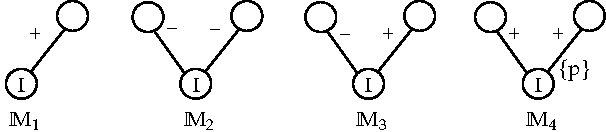
\includegraphics{fig-pnl}
\end{center}
The following holds:
\begin{itemize}
\item$\M_1$: $I$ have a friend where $\neg p$: $\M_1, I \Vdash \dplus\neg p$;
\item$\M_2$: All $my$ enemies do not believe in $p$: $\M_2, I \Vdash \bminus\neg p$;
\item$\M_3$: $I$ have an enemy: $\M_3, I \Vdash \dminus\top$;
\item$\M_4$: Everybody has a friend where $p$: $\M_4, \ag \Vdash  [A ]  \dplus p$ for any agent $\ag$.
\end{itemize} 
 \end{example}


\subsection{Playing with models}\label{sec:game-semantics}
Before starting playing, remember that in a \PNL-model $\M$, every agent $\ag$ has a name $i$, \ie, there exists $i\in N$ s.t. $\g(i)=\ag$. Hence, from now on, we will internalise the nominals, identifying an agent $\ag$ with its respective nominal $i$.

The  \emph{semantic game} is played over a \PNL-model $\M=(\A,\R^+,\R^-,\V,\g)$ by two
players, \Me (or \Ic) and \You, who argue about the truth of a formula $ F $ at an
agent $i$. At each stage of the game, one player acts as \emph{proponent}, while the
other acts as \emph{opponent} of the claim that  $ F $ is true at 
$i$. 

We represent the situation where \Ic am the proponent (and \You are the
opponent) by the \emph{game state} $\mathbf{P}, i: F $, and the situation
where \Ic am the opponent (and \You are the proponent) by $\mathbf{O},
i: F $. 

We call a game state \emph{elementary} if its involved formula is elementary. For a game state $g$, we denote the game starting at $g$ over the model $\M$ by $\mathbf{G}_\M(g)$.

The game over a \PNL-model $\M$ proceeds by reducing the involved formula $ F $ to an elementary formula by following the rules described in Figure~\ref{fig:game-rules}.\footnote{The outcome of the game state $\mathbf{Q},k:R^{\pm}(i,j)$ is independent of $k$ (it only depends on the underlying model $\M$). Hence, we write 
        $\mathbf{Q},\_:R^\pm(i,j)$ instead of $\mathbf{Q},k:R^\pm(i,j)$.\label{foot:R}}


\begin{figure}
~~~\resizebox{.92\textwidth}{!}{
\begin{minipage}[t]{\textwidth}
    \hrulefill
\begin{description}
\item[$(\mathbf{P}_\wedge)$] At $\mathbf{P},  i :  F _1\wedge  F _2$, \You
    choose between  $\mathbf{P}, i : F _1$ and 
    $\mathbf{P}, i : F _2$ to continue the game. \\
\item[$(\mathbf{O}_\wedge)$] \vspace{-2mm}At $\mathbf{O},  i :
     F _1\wedge  F _2$, \Ic choose between $\mathbf{O}, i : F _1$
    and $\mathbf{O}, i : F _2$ to continue the game. \\

\item[$(\mathbf{P}_\vee)$] At $\mathbf{P},  i :  F _1\vee  F _2$, \Ic choose between $\mathbf{P}, i : F _1$ and $\mathbf{P}, i : F _2$ to continue the game.\\
\item[$(\mathbf{O}_\vee)$] \vspace{-2mm}At $\mathbf{O},  i :  F _1\vee  F _2$, \You choose between $\mathbf{O}, i : F _1$ and $\mathbf{O}, i : F _2$ to continue the game.\\

\item[$(\mathbf{P}_\neg)$] At $\mathbf{P},  i : \neg  F $, the game continues with $\mathbf{O},  i :  F $.\\
\item[$(\mathbf{O}_\neg)$] \vspace{-2mm}At $\mathbf{O},  i : \neg  F $, the game continues with $\mathbf{P}, i :  F $.\\
    \item[$(\mathbf{P}_{\Diamond^\pm})$] At $\mathbf{P}, i: \Diamond^\pm  F $, \Ic choose a nominal $j$, and \You decide whether the game ends in the state $\mathbf{P},\_:R^\pm(i,j)$ or continues with $\mathbf{P},j:  F $.\\
        \item[$(\mathbf{O}_{\Diamond^\pm})$] \vspace{-2mm} At $\mathbf{O},i: \Diamond^\pm  F $, \You choose  $j$, and \Ic choose between $\mathbf{O},\_:R^\pm(i,j)$ and $\mathbf{O},j: F $.\\
\item[$(\mathbf{P}_{[A]})$] At $\mathbf{P},i: [A] F $, \You choose a nominal $j$ and the game continues with $\mathbf{P},j: F $.\\
\item[$(\mathbf{O}_{[A]})$] \vspace{-2mm} At $\mathbf{O},i: [A] F $, \Ic choose a nominal $j$, and the game continues with $\mathbf{O},j:  F $.\\
\item[$(\mathbf{P}_{el})$] Let $ F _{e}$ be an elementary formula. \Ic win and \You lose at $\mathbf{P}, i : F _{e}$ iff $~\mathbb{M}, i  \models  F _{e}$. Otherwise, \You win and \Ic lose.\\
\item[$(\mathbf{O}_{el})$] \vspace{-2mm}At $\mathbf{O}, i  :  F _{e}$, \Ic win and \You lose iff $\mathbb{M}, i \not \models  F _{e}$. Otherwise, \You win and \Ic lose.\\
\end{description}
    \hrulefill
\end{minipage}
}
\caption{Semantic game given a \PNL-model $\M$.\label{fig:game-rules}}
\end{figure}

In general, every two-person, zero-sum, win-lose game is usually represented by
a game tree. In our
case, the root of the game tree representing the game
$\mathbf{G}_\mathbb{M}(g)$ is $g$. The children of each node in the game tree
are exactly the possible choices of the corresponding player. For instance, if
$h=\mathbf{P},  i :  F _1\wedge  F _2$ appears in the game tree, then its
children are $\mathbf{P}, i : F _1$ and $\mathbf{P}, i : F _2$. Each node in
the tree is labelled either ``I'', or ``Y'', depending on which player is to
move in the corresponding game state, and we label 
the nodes  $\mathbf{P},  i : \neg  F $ and $\mathbf{O},  i :
\neg  F $ with ``I'' (even though there is no choice involved in these game
states). For instance, the node corresponding to the game state $h$ above is
``Y'', since it is \Your choice in $\mathbf{P}: F _1\wedge  F _2$. The leaves
of the tree receive the label of the winning player. 
A \emph{run} of the game is a maximal path through the game tree.

Now we are ready to define winning strategies and state the main result of this section:
the adequacy of the proposed game semantics with respect to the Kripke semantics for \PNL.

\begin{definition}
    A \emph{strategy} for \Me in the game $\mathbf{G}_\M(g)$ is a subtree $\sigma$ of the associated game tree such that: 
 \textbf{(1)} $g\in \sigma$,
 \textbf{(2)} if $h\in \sigma$ is a node labelled ``Y'', then all children of $h$ are in $\sigma$,
 \textbf{(3)} if $h\in \sigma$ is a node labelled ``I'', then exactly one child of $h$ is in $\sigma$.
The strategy $\sigma$ is called \emph{winning} if all leaves in the tree $\sigma$ are labelled ``I''. (Winning) strategies for \You are defined dually.
\end{definition}

\begin{theorem}[Adequacy - semantic games~\cite{LPAR2024:Reasoning_About_Group_Polarization}]%\label{winningstrategy}
\label{th:adequacy}
Let $\M$ be a \PNL-model, $\ag$ an agent with nominal $i$, and $F$ a formula.

\noindent\textbf{(1)} \Ic have a winning strategy for $\mathbf{G}_\M(\mathbf{P}, i:F)$ iff $\M,\ag \models F$. 

\noindent\textbf{(2)} \You have a winning strategy for $\mathbf{G}_{\M}(\mathbf{P}, i:F)$ iff $\M,\ag\not \models F$.
\end{theorem}

 
  \begin{example}[\cite{LPAR2024:Reasoning_About_Group_Polarization}]\label{ex:balance}
     Let 
     $ \mathbf{(4B)} = 
        ((\dplus\dplus p \vee \dminus\dminus p)\to \dplus p) \wedge
        ((\dplus \dminus p \vee \dminus\dplus p)\to \dminus p)
    $. This formulas 
    specifies \emph{local balance} \cite{DBLP:journals/logcom/PedersenSA21}
    and   captures the idea that 
``the enemy of my enemy is my friend'',  ``the friend
of my enemy is my enemy'',  and ``the friend of my friend is my friend''.
 %A collectively connected network where $[A]4B$ holds is a polarized network, 
%where agents can be divided into two opposing groups \cite{balance}.
    $\Ic$ have a winning strategy for the game $\bfP,\ag : 4B$
    on $\bbM_1$ 
    while $\You$ have a winning strategy for the same game on $\bbM_2$ where (omitting self-loops for $\R^+$):

	\vspace{0,4cm}
    \begin{tabularx}{.6\textwidth}{ X X X X X }
        $\bbM_1=$ & \parbox[c]{\hsize}{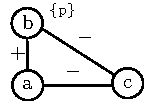
\includegraphics[scale=0.85]{fig2}} & \qquad &
        $\bbM_2=$ & \parbox[c]{\hsize}{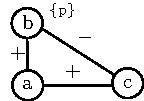
\includegraphics[scale=0.85]{fig3}} 
    \end{tabularx}

	\vspace{0,4cm}
    For $\bbM_1$, in the first conjunct, \Ic pick ($\bfP_\vee$)
    $\dplus p$ and then $\b$ in ($\bfP_{\dplus}$); for the second conjunct,
    \Ic pick the first disjunction in $F=(\dplus \dminus p \vee \dminus\dplus p)\to \dminus p)$
    where, in any of \Your choices ($\bfP_{\neg}$ followed by $\bfO_{\vee}$ and 
    $\bfO_{\Diamond^{\pm}}$), \Ic  win all the elementary states. 
    For $\bbM_2$, \Ic do not have a winning strategy 
    for the  second conjunct: \Ic can neither win $\dminus p$ (no $\R^{-}$ successor), 
    nor the first disjunct in  $F$ above since, after $\bfP_{\neg}$, 
    \You choose  ($\bfO_{\vee}$) 
    $\dplus\dminus p$ and select $\mathsf{c}$ and then $\b$ ($\bfO_{\Diamond^{\pm}}$)
    where $p$ holds and \You win. See the complete game in our tool \cite{tool}. 
	%\todo{Appendix}
% and \Cref{ap:examples}.
\end{example}

\subsection{Playing all models}
We now leverage semantic games to \PNL-provability games. The key observation is that the rules of the semantic game remain independent of the underlying model, except at the level of elementary game states.

The {\em provability game}
$\mathbf{DG}(\mathbf{P},i:F )$ can be thought of as \Me and \You playing all
semantic games $\mathbf{G}(\mathbf{P},i:F )$ over all \PNL-models $\M$
simultaneously. We point out that  the rules of the semantic game do not depend on the structure
of $\M$ but merely on $F $. Truth degrees are only needed at the atomic level
to determine who wins the particular run of the game. This allows us to require
players to play ``blindly'', \ie, without explicitly referencing  a model $\M$.
Clearly, if \Ic have a winning strategy in such a game, then \Ic can win in
$\mathbf{G}_\M(\mathbf{P},i:F )$, for every $\M$, making this strategy an
adequate witness of logical validity. 

Provability game states are finite multisets of the game states
defined in Section \ref{sec:game-semantics}. We denote by $g_1 \bigvee ... \bigvee g_n$ 
 the provability game state $\{g_1,...,g_n\}$.
% , but keep the convenient notation $g\in D$ if $g$ is in the  multiset $D$. 
We write $D_1 \bigvee D_2$ for the
multiset sum $D_1+D_2$ and $D\bigvee g$ for $D+\{g\}$. A provability state is
called \emph{elementary} if all its game states are elementary.
We use $\mathbf{DG}(D)$ to denote the provability game starting at $D$. 

\begin{definition}\label{def:win}
Let $D^{el}$ denote the provability state consisting of the elementary game
states of $D$. \Ic win and \You lose at $D$ if for every \PNL-model there is
a game state in $D^{el}$ where \Ic win the corresponding semantic game. 
\end{definition}

In the provability game, \Ic additionally take the
role of a \emph{scheduler}, deciding which game  is to be played next. We
signal the chosen game state by underlining it as in $\underline{g}$.


\begin{figure}
\resizebox{0.93\textwidth}{!}{
\begin{minipage}[t]{\textwidth}
\hrulefill
\begin{description}
%\item[(End)] If no state in $D$ is underlined, \Ic can end the game and $D$ becomes terminal.
\item[(Dupl)] If no state in $D$ is underlined,
    %and $D$ is not terminal, 
    \Ic can choose a non-elementary $g\in D$ and the game continues with $D\bigvee g$.
\item[(Sched)] If no state in $D=D'\bigvee g$ is underlined,
    %and $D$ is not terminal, 
    and $g$ is non-elementary, 
    \Ic can choose to continue the game  with $D'\bigvee \underline{g}$.
\item[(Move)] If $D=D'\bigvee \underline{g}$ then the player who is to move in
    the semantic game $\mathbf{G}(g)$ at $g$ makes a legal move to the game
    state $g'$ and the game continues with $D' \bigvee g'$.
\item[(End)]
    The game ends if there are no non-elementary game states left in $D$, or if
    no game state is underlined and \Ic win according to
    Definition~\ref{def:win}. Otherwise, \Ic must move according to
    \textbf{(Dupl)} or \textbf{(Sched)}.
\end{description}
\hrulefill
\end{minipage}
}
\caption{Rules for the provability game\label{fig:dg-rules}.}
\end{figure}

\begin{definition}\label{def:dg}
    The rules of the provability game are in \Cref{fig:dg-rules}.
%\noindent %Additionally, we require that if no game state of $D$ is underlined, \Ic must move according to 
%\textbf{(End)}, 
%\textbf{(Dupl)} or \textbf{(Sched)}. \textbf{(Dupl)} is referred to as the \emph{duplication rule} and \textbf{(Sched)} as the \emph{scheduling}, or \emph{underlining rule}.
Infinite runs, and runs that end in elementary provability states where \Ic do not win according to Definition~\ref{def:win}, are winning for \You and losing for \Me.  \textbf{(Dupl)} is referred to as the \emph{duplication rule} and \textbf{(Sched)} as the \emph{scheduling}, or \emph{underlining rule}.
\end{definition}

\begin{theorem}[Adequacy - provability games~\cite{LPAR2024:Reasoning_About_Group_Polarization}]
\label{thm:adeq} \Ic have a winning strategy in $\mathbf{DG}(D)$  iff for every  \PNL-model $\mathbb{M}$, there is some $g\in D$ such that \Ic have a winning strategy in $\mathbf{G}_\mathbb{M}(g)$.
\end{theorem}

\begin{corollary}
The formula $F $ is  \PNL-valid iff \Ic have a winning strategy in $\mathbf{DG}(\mathbf{P},i:[A]F )$.
\end{corollary}

\begin{example}
Consider  the game $\mathbf{P},i: p \vee \neg p$.
\Ic duplicate the game state in the first round and the
game continues with the provability state $\mathbf{P},i: p \vee \neg
p\bigvee \mathbf{P},i: p \vee \neg p$. 

Now \Ic move to $\mathbf{P},i: p$ in the
first subgame and to $\mathbf{P},i:\neg p$ in the second. After a role switch
in the second subgame, the final state is $\mathbf{P},i: p \bigvee
\mathbf{O},i: p$, where \Ic win regardless of the underlying model.
\end{example}

\subsection{From games to proofs}\label{sec:proofs}

Theorems~\ref{th:adequacy} and \ref{thm:adeq} establish that winning strategies for \Me in the provability game correspond to the validity of formulas. In this section, we extend this result to proof systems by introducing a sequent calculus, 
$\DS$, where proofs correspond to \My's winning strategies in the provability game.

{\em Labelled nominal formulas} are either \emph{labelled formulas} of
the form $i: F $ or \emph{relational atoms} of the form $R(i,j)$,
where $i$ and $j$ are nominals and $ F $ is a \PNL~formula.%
\footnote{Observe that here we are abusing the notation, identifying $k:R(i,j)$ with $R(i,j)$ -- see Footnote~\ref{foot:R}.} \emph{Labelled sequents} have the form $\Gamma \seq \Delta$, where
$\Gamma,\Delta$ are multisets containing labelled nominal formulas.

Starting with sequents, every provability state of the form
\begin{center}
$
\mathbf{O},i_1:  F_1\bigvee \ldots \bigvee \mathbf{O},i_n:  F_n\bigvee\mathbf{P},j_1: G_1 \bigvee \ldots \bigvee \mathbf{P},j_m: G_m
$
\end{center}
 can be rewritten as the labelled sequent $\Gamma \seq \Delta$ where
$
\Gamma =\{i_1: F_1, \ldots, i_n: F_n\}\mbox{ and } \Delta =\{j_1: G_i,\ldots,j_m: G_m\}
$. 
In what follows, we will not distinguish between provability states and their corresponding labelled sequent. For example,
the provability game state
$\mathbf{O},i:(\dplus\dplus p \vee \dminus\dminus p)\bigvee\mathbf{P},i: \dplus p$
will be identified with the sequent  
$i:(\dplus\dplus p \vee \dminus\dminus p)\seq i: \dplus p$.

The inference rules must be tailored in such a way that {\em
proofs} in the sequent system match exactly \My\  {\em winning strategies} in
the provability game. This means that the user of the proof system takes the
role of \Me, scheduling game states and choosing moves in \I-states. 
Moreover, {\em provability} in the proof system should correspond to {\em
validity} in the game. For that,  it is necessary to establish the
formal relationship between elementary game states and logical axioms.


\begin{lemma}[\cite{LPAR2024:Reasoning_About_Group_Polarization}]\label{lemma:init}
    Let $\Gamma\seq \Delta$ be composed of elementary game states only. \Ic win the provability game in $\Gamma \seq \Delta$ iff one of the following holds\footnote{\label{foot:sym}Since relations are symmetric, we will identify $R^\pm(i,j)$ with  $R^\pm(j,i)$.} 
%\begin{itemize}
    
    \noindent\textbf{i.} $R^-(i,i)\in\Gamma$ or $R^+(i,i)\in\Delta$ for some $i$;

    \noindent\textbf{ii.} $\{R^+(i,j),R^-(i,j)\}\subseteq\Gamma$ for some $i\not=j$;

    \noindent\textbf{iii.} $\Gamma\cap\Delta\not=\emptyset$.
\end{lemma}
Figure~\ref{fig:calculus} presents the labelled sequent systems $\DS$ with the standard initial axiom and structural/propositional  rules. The modal  rules and the relational rules $sym$ and  $ref\pm$  coincides with the modal rules originally presented by Vigan\`{o} in~\cite{Vigano:2000}, adapted to multi-relational modal logics. 
%
It is routine to show that the rule $no$ in Figure~\ref{fig:calculus} correspond to the non-overlapping  axiom
$
\forall i,j. \neg(R^+(i,j)\wedge R^-(i,j)) 
$.

The following result immediately implies that the provability game $\mathbf{DG}$ is adequate with respect to the calculus $\DS$.

\begin{theorem}[Adequacy - sequent system~\cite{LPAR2024:Reasoning_About_Group_Polarization}]\label{thm:adequacy-sequent}
\Ic have a winning strategy in the provability game $\mathbf{DG}(\Gamma\seq\Delta)$  iff $\Gamma\seq\Delta$ is provable in $\DS$. 
\end{theorem}

Let us write $\models_\PNL \Gamma \Rightarrow \Delta$ iff for every \PNL-model there is some $i:F \in \Gamma$ such that $\M,\g(i)\not\models F$, or there is some $i:G \in \Delta$ such that $\M,\g(i)\models G$. We have the following consequence of Theorems~\ref{th:adequacy},~\ref{thm:adeq}, and~\ref{thm:adequacy-sequent}: 

\begin{corollary}
Let $\Gamma,\Delta$ be multisets of labelled formulas. Then $\models_\PNL\Gamma \Rightarrow \Delta$ iff there is a proof of $\Gamma \Rightarrow \Delta$ in $\DS$. In particular, $ F $ is \PNL-valid iff there is a proof of $\Rightarrow  F $ in $\DS$.
\end{corollary}

\begin{figure}[ht]
    \begin{center}
\resizebox{.85\textwidth}{!}{
\begin{minipage}[t]{\textwidth}
	\headline{\sc Axiom and Structural Rules}
	
	\medskip

    \begin{center}
 \begin{prooftree}
        \hypo {}
        \infer1 [$init$]{\Gamma, i: F_{el} \Rightarrow  \Delta, i: F_{el}}
        \end{prooftree}
\qquad
 \begin{prooftree}
        \hypo {\Gamma, i:  F, i:  F  \Rightarrow  \Delta}
        \infer1 [$(L_c)$]{\Gamma, i:  F  \Rightarrow  \Delta}
        \end{prooftree}        
		\qquad
        \begin{prooftree}
        \hypo {\Gamma \Rightarrow  i:  F ,i:  F ,\Delta}
        \infer1 [$(R_c)$]{\Gamma \Rightarrow  i:  F , \Delta}
        \end{prooftree}
    \end{center}
        
\headline{\sc Propositional Rules}
\begin{center}
        \begin{prooftree}
        \hypo {\Gamma \Rightarrow i:  F , \Delta}
        \infer1 [\((L_\neg)\)]{\Gamma, i: \neg  F  \Rightarrow \Delta}
        \end{prooftree}
  \qquad
  \begin{prooftree}
        \hypo {\Gamma, i:   F  \Rightarrow \Delta}
        \infer1[\((R_\neg)\)]{\Gamma \Rightarrow i: \neg   F , \Delta}
        \end{prooftree}

\bigskip

        \begin{prooftree}
        \hypo {\Gamma, i:  F  \Rightarrow \Delta}
        \hypo{\Gamma, i: G \Rightarrow \Delta}
        \infer2 [\((L_\vee)\)]{\Gamma, i:  F  \vee  G \Rightarrow \Delta}
        \end{prooftree}
        \qquad
        \begin{prooftree}
        \hypo {\Gamma \Rightarrow i:   F , \Delta}
        \infer1[\((R_\vee^1)\)]{\Gamma \Rightarrow i:   F  \vee  G, \Delta}
        \end{prooftree}
        \qquad 
        \begin{prooftree}
        \hypo {\Gamma \Rightarrow i:  G, \Delta}
        \infer1[\((R_\vee^2)\)]{\Gamma \Rightarrow i:   F  \vee  G, \Delta}
        \end{prooftree}
        \bigskip

        \begin{prooftree}
        \hypo {\Gamma, i:  F  \Rightarrow \Delta}
        \infer1 [\((L_\wedge^1)\)]{\Gamma, i:  F  \wedge  G \Rightarrow \Delta}
        \end{prooftree}
       \qquad
    	\begin{prooftree}
        \hypo {\Gamma, i: G \Rightarrow \Delta}
        \infer1 [\((L_\wedge^2)\)]{\Gamma, i:  F  \wedge  G \Rightarrow \Delta}
        \end{prooftree}
       \qquad
       \begin{prooftree}
        \hypo {\Gamma \Rightarrow i:   F , \Delta}
        \hypo {\Gamma \Rightarrow i:  G, \Delta}
        \infer2[\((R_\wedge)\)]{\Gamma \Rightarrow i:   F  \wedge  G, \Delta}
        \end{prooftree}
                
    \end{center}
\headline{\sc Modal Rules}
\begin{center}
         \begin{prooftree}
        \hypo {\Gamma, R^\pm(i,j) \Rightarrow \Delta}
        \infer1 [\((L_{\Diamond^\pm})_1\)]{\Gamma, i: \Diamond^\pm  F \Rightarrow \Delta}
        \end{prooftree}
       \qquad
       \begin{prooftree}
        \hypo {\Gamma, j: F  \Rightarrow \Delta}  
        \infer1 [\((L_{\Diamond^\pm})_2\)]{\Gamma, i: \Diamond^\pm  F \Rightarrow \Delta}
        \end{prooftree}
      \bigskip
      
      \begin{prooftree}
        \hypo {\Gamma \Rightarrow R^\pm(i,j), \Delta}
        \hypo {\Gamma \Rightarrow j:  F , \Delta}
        \infer2 [\((R_{\Diamond^\pm})\)]{\Gamma\Rightarrow i: \Diamond^\pm  F ,\Delta}
        \end{prooftree}
        \quad
        \begin{prooftree}
        \hypo {\Gamma, j:  F  \Rightarrow \Delta}
        \infer1 [$(L_{[A]})$]{\Gamma,  i:[A] F  \Rightarrow \Delta}
        \end{prooftree}
        \quad
        \begin{prooftree}
        \hypo {\Gamma \Rightarrow  j:  F , \Delta}
        \infer1 [$(R_{[A]})$]{\Gamma\Rightarrow  i:[A] F , \Delta}
        \end{prooftree}

    \end{center}

        
\headline{\sc Relational Rules}
\begin{center}
         \begin{prooftree}
        \hypo {\Gamma \Rightarrow  \Delta, R^{\pm}(j,i)}
        \infer1 [$sym$]{\Gamma \Rightarrow  \Delta, R^{\pm}(i,j)}
        \end{prooftree}
        \qquad
\begin{prooftree}
        \hypo { }
        \infer1 [$ref+$]{\Gamma\Rightarrow  \Delta, R^{+}(i,i)}
        \end{prooftree}
        \bigskip

\begin{prooftree}
        \hypo { }
        \infer1 [$ref-$]{\Gamma, R^{-}(i,i)\Rightarrow  \Delta}
        \end{prooftree}
        \qquad
        \begin{prooftree}
        \hypo {\Gamma \Rightarrow  \Delta, R^+(i,j)}
        \hypo {\Gamma \Rightarrow  \Delta, R^-(i,j)}
        \infer2 [$no$]{\Gamma \Rightarrow  \Delta}
        \end{prooftree}
    \end{center}
        
\end{minipage}
}
\end{center}
\vspace{-0.3cm}
%        \begin{prooftree}
%        \hypo {\Gamma, R^+(i,j) \Rightarrow  \Delta}
%        \hypo {\Gamma, R^-(i,j) \Rightarrow  \Delta}
%        \infer2 [$cc$]{\Gamma \Rightarrow  \Delta}
%        \end{prooftree}
 \caption{The proof system $\DS$.
     %is formed by the initial axiom plus the structural, propositional, relational and modal rules.  
     In the rule init, $F_{el}$ denotes an
elementary formula. In the rules   $(L_{\Diamond^\pm})_1$,
$(L_{\Diamond^\pm})_2$, and $(R_{[A]})$,  the nominal $j$ is fresh.
 The rule
$R_{\meddiamondminus}$ has the proviso that $i\neq j$.  \label{fig:calculus} } 
\end{figure}

Proving cut-admissibility of labelled systems can be cumbersome due to the presence of relational rules. %(see \eg\ \cite{negri99aml}).
%Moreover, it is usually done in a case-by-case analysis, tailored for each system (see \eg\ \cite{negri99aml}). 
%
In~\cite{DBLP:journals/apal/MarinMPV22}, a systematic procedure for
transforming axioms into rules was presented, based on {\em focusing} and {\em
polarities}~\cite{andreoli92jlc}. This procedure not only allows for 
generalizing different approaches for transforming axioms into sequent
rules present in the literature~\cite{Sim94,Vigano:2000,Neg05}, but it also provides 
a uniform way of proving cut-admissibility for the resulting systems.

The cut-admissibility result for $\DS$ is a particular instance of the general result in~\cite{DBLP:journals/apal/MarinMPV22}.
\begin{theorem}[\PNL-cut]\label{thm:cut}
The following cut rule is admissible in $\DS$

\vspace{0.15cm}
\qquad\qquad\qquad\qquad$
\infer[cut]{\Gamma\seq\Delta}{\Gamma\seq\Delta,i: F  & i: F ,\Gamma\seq\Delta}
$
\end{theorem}
%For the reader interested in understanding focusing, polarities and the axioms-as-rules approach, we have added a gentle introduction in Appendix~\ref{app:focusing}. We refer to~\cite{DBLP:journals/apal/MarinMPV22} for further reading on the topic.
As a consequence, %of Theorem~\ref{thm:cut}, 
$\DS$ is consistent, since the only rule that can be applied in an empty sequent is $no$, and it is routine to show that it does not trivialise derivations. 




\subsection{Discussion -- part II}\label{subsec:conc2}
%!TEX root = CSL.tex

This work opens up several promising directions for future exploration.

In terms of variations on the present work, it would be interesting to explore extensions of \PNL\ that relax symmetry assumptions, enabling the representation of scenarios where an agent $a$ can influence the opinion of agent $b$, but not vice versa. Another potential direction involves incorporating the concept of a ``budget,'' as introduced in the game discussed in the first part of this paper~\cite{DBLP:conf/tableaux/LangOPF19}, to model situations where proponents and opponents operate under a limited amount of political capital. In such scenarios, adding or modifying relationships could reduce this capital.

To formalize this idea, preferences for minimizing the expenditure of political capital could be expressed through a combination of \PNL\ with a suitable choice logic -- a framework where preferences are explicitly definable at the object level. Semantic games for choice logics have been explored in~\cite{Freiman2023TruthLogic}, and the extension of game-induced choice logic (\textbf{GCL}) to a provability game and proof system was proposed in~\cite{Freiman2023}. 
%Investigating these integrations offers a compelling avenue for further research.

Another particularly interesting avenue is extending the semantic-provability-proof system approach to other logics characterized by Kripke semantics. For instance, it would be worthwhile to investigate games for logics that involve model-change modalities~\cite{DBLP:journals/logcom/Velazquez-Quesada17,DBLP:journals/igpl/PerrotinV21} or dynamic modalities~\cite{DBLP:journals/synthese/BenthemGL08}. Initial progress in this direction was made in~\cite{LPAR2024:Reasoning_About_Group_Polarization}, where we showed how the global link-adding and local link-changing modalities from~\cite{DBLP:journals/logcom/PedersenSA21} (inspired by sabotage modal logic~\cite{DBLP:journals/igpl/ArecesFH15,DBLP:journals/logcom/AucherBG18,DBLP:journals/logcom/BenthemLSY23}) can be incorporated into our framework.

This extension is motivated by the study of social learning and opinion dynamics, which aim to understand how specific social factors influence the acceptance or rejection of opinions. Such models can provide insights into scenarios like consensus, polarization, and fragmentation. In these contexts, positive and negative relationships between agents are not fixed; they evolve over time. For example, enemies may reconcile, new friendships or agreements may form, or agents may develop disagreements. Exploring these dynamics within our framework offers a compelling direction for future research. 

Finally, we are particularly interested in exploring the application of this framework to develop games for constructive and intuitionistic modal logics~\cite{Fitch,plotkin:stirling:86,Sim94,DBLP:journals/sLogica/BiermanP00}. The constructive logic $\CK$ stands out as a promising candidate due to its intuitive semantics and straightforward sequent system. The main challenge lies in adapting the classical approach presented here to an intuitionistic setting. The framework introduced in the first part of this paper could prove instrumental in addressing this challenge.

Building on ideas from~\cite{DBLP:conf/eumas/AcclavioC23}, we aim to establish a correspondence between winning innocent strategies in games played on Hyland-Ong arenas~\cite{DBLP:journals/iandc/HylandO00} and proofs in these constructive logics. This correspondence would deepen the connection between game semantics and constructive modal reasoning, opening new avenues for further study.

 
\bibliography{references}
\end{document}

\end{document}
